%%%%%%%%%%%%%%%%%%%%%%%%%%%%%%%%%%%%%%%%%%%%%%%%%%%%%%%%%%%%%%%%%%%%%%%%%%%%%
%%% LaTeX-Rahmen fuer das Erstellen von Bachelorarbeiten
%%%%%%%%%%%%%%%%%%%%%%%%%%%%%%%%%%%%%%%%%%%%%%%%%%%%%%%%%%%%%%%%%%%%%%%%%%%%%

%%%%%%%%%%%%%%%%%%%%%%%%%%%%%%%%%%%%%%%%%%%%%%%%%%%%%%%%%%%%%%%%%%%%%%%%%%%%%
%%% allgemeine Einstellungen
%%%%%%%%%%%%%%%%%%%%%%%%%%%%%%%%%%%%%%%%%%%%%%%%%%%%%%%%%%%%%%%%%%%%%%%%%%%%%

\documentclass[twoside,12pt,a4paper]{report}
%\usepackage{reportpage}
\usepackage[main=ngerman]{babel}
\usepackage{graphics, graphicx}
\usepackage[utf8]{inputenc}
\usepackage{latexsym}
\usepackage[margin=10pt,font=small,labelfont=bf]{caption}
\usepackage{subfig}
\usepackage{amsmath}
\usepackage{placeins}

\textwidth 14cm
\textheight 22cm
\topmargin 0.0cm
\evensidemargin 1cm
\oddsidemargin 1cm
%\footskip 2cm
\parskip0.5explus0.1exminus0.1ex

% Kann von Student auch nach pers\"onlichem Geschmack ver\"andert werden.
\pagestyle{headings}

\sloppy

\begin{document}
	
	%%%%%%%%%%%%%%%%%%%%%%%%%%%%%%%%%%%%%%%%%%%%%%%%%%%%%%%%%%%%%%%%%%%%%%%%%%%%
	%%% hier steht die neue Titelseite 
	%%%%%%%%%%%%%%%%%%%%%%%%%%%%%%%%%%%%%%%%%%%%%%%%%%%%%%%%%%%%%%%%%%%%%%%%%%%%
	
	\begin{titlepage}
		\begin{center}
			{\LARGE Eberhard Karls Universit"at T"ubingen}\\
			{\large Mathematisch-Naturwissenschaftliche Fakult"at \\
				Wilhelm-Schickard-Institut f"ur Informatik\\[4cm]}
			{\huge Bachelorarbeit Informatik\\[2cm]}
			{\Large\bf  Titel der Arbeit\\[1.5cm]}
			{\large Tolga Demir}\\[0.5cm]
			Datum\\[3cm]
			\begin{center}{\small\bf Gutachter}\\[0.5cm]
				{\large Prof. Andreas Zell}\\
				{\footnotesize Wilhelm-Schickard-Institut f\"ur Informatik\\
					Universit"at T"ubingen}	\end{center}
			
			
			
		\end{center}
	\end{titlepage}
	
	%%%%%%%%%%%%%%%%%%%%%%%%%%%%%%%%%%%%%%%%%%%%%%%%%%%%%%%%%%%%%%%%%%%%%%%%%%%%
	%%% Titelr"uckseite: Bibliographische Angaben
	%%%%%%%%%%%%%%%%%%%%%%%%%%%%%%%%%%%%%%%%%%%%%%%%%%%%%%%%%%%%%%%%%%%%%%%%%%%%
	
	\thispagestyle{empty}
	\vspace*{\fill}
	\begin{minipage}{11.2cm}
		\textbf{Nachname, Vorname:}\\
		\emph{Titel der Arbeit}\\ Bachelorarbeit Bioinformatik\\
		Eberhard Karls Universit"at T"ubingen\\
		Bearbeitungszeitraum: von-bis
	\end{minipage}
	\newpage
	
	%%%%%%%%%%%%%%%%%%%%%%%%%%%%%%%%%%%%%%%%%%%%%%%%%%%%%%%%%%%%%%%%%%%%%%%%%%%%%
	%%% Erklaerung
	%%%%%%%%%%%%%%%%%%%%%%%%%%%%%%%%%%%%%%%%%%%%%%%%%%%%%%%%%%%%%%%%%%%%%%%%%%%%%
	\thispagestyle{empty}
	
	\section*{Selbst\"andigkeitserkl\"arung}
	
	Hiermit versichere ich, dass ich die vorliegende Bachelorarbeit 
	selbst\"andig und nur mit den angegebenen Hilfsmitteln angefertigt habe und dass alle Stellen, die dem Wortlaut oder dem 
	Sinne nach anderen Werken entnommen sind, durch Angaben von Quellen als 
	Entlehnung kenntlich gemacht worden sind. 
	Diese Bachelorarbeit wurde in gleicher oder \"ahnlicher Form in keinem anderen 
	Studiengang als Pr\"ufungsleistung vorgelegt. 
	
	\vskip 3cm
	
	Ort, Datum	\hfill Unterschrift \hfill 
	\newpage
	
	%%%%%%%%%%%%%%%%%%%%%%%%%%%%%%%%%%%%%%%%%%%%%%%%%%%%%%%%%%%%%%%%%%%%%%%%%%%%
	
	\pagenumbering{roman}
	\setcounter{page}{1}
	
	%%%%%%%%%%%%%%%%%%%%%%%%%%%%%%%%%%%%%%%%%%%%%%%%%%%%%%%%%%%%%%%%%%%%%%%%%%%%
	%%% Seite I: Zusammenfassug, Danksagung
	%%%%%%%%%%%%%%%%%%%%%%%%%%%%%%%%%%%%%%%%%%%%%%%%%%%%%%%%%%%%%%%%%%%%%%%%%%%%
	
	
	\section*{Zusammenfassung}
	
	Hier kommt die Zusammenfassung hin!!!
	
	\newpage
	
	\section*{Danksagung}
	Mein Dank gilt Prof. Zell, der diese Bachelorarbeit engagiert ermöglicht und begleitet hat. \\
	Weiterhin möchte ich mich herzlich beim Wohnheim Rechberghaus bedanken für die Bereitstellung einer Werkstatt. Ohne diese Hilfe wären mir manche Arbeiten am Roboter kaum möglich gewesen. 
	\cleardoublepage
	
	%%%%%%%%%%%%%%%%%%%%%%%%%%%%%%%%%%%%%%%%%%%%%%%%%%%%%%%%%%%%%%%%%%%%%%%%%%%%%
	%%% Inhaltsverzeichnis
	%%%%%%%%%%%%%%%%%%%%%%%%%%%%%%%%%%%%%%%%%%%%%%%%%%%%%%%%%%%%%%%%%%%%%%%%%%%%%
	
	\renewcommand{\baselinestretch}{1.3}
	\small\normalsize
	
	\tableofcontents
	
	\renewcommand{\baselinestretch}{1}
	\small\normalsize
	
	\cleardoublepage
	
	
	%%%%%%%%%%%%%%%%%%%%%%%%%%%%%%%%%%%%%%%%%%%%%%%%%%%%%%%%%%%%%%%%%%%%%%%%%%%%%
	%%% Der Haupttext, ab hier mit arabischer Numerierung
	%%% Mit \input{dateiname} werden die Datei `dateiname' eingebunden
	%%%%%%%%%%%%%%%%%%%%%%%%%%%%%%%%%%%%%%%%%%%%%%%%%%%%%%%%%%%%%%%%%%%%%%%%%%%%%
	
	\pagenumbering{arabic}
	\setcounter{page}{1}
	
	\chapter{Einführung}
	
	% ganze Kapitel 5 Seiten max
	\section{Autonome Mobile Roboter}
	Mobile Roboter werden für eine breite Bandbreite an Arbeiten eingesetzt, darunter die Erkundung von menschenfeindlichen Umgebungen, das Verrichten von Arbeiten in diesen oder als Service-Roboter z.B. zum Rasenmähen oder Staubsaugen.\\
	Die Bezeichnung autonom meint hierbei, dass die Roboter ihre Aufgaben (fast-) selbstständig erledigen. Dazu gehören neben der reinen Tätigkeit auch Themen wie das Fahren, Erfassen von Zielen, Erstellen von Karten ihrer Umgebung und zurecht finden in unbekanntem Terrain. \\
	Mobile Roboter sind seit den 1960ern ein Feld intensiver Forschung mit vielen Applikationen in der Industrie. Seit den 2000ern werden eine Vielzahl von verschiedenen Mobilen Robotern für die Industrie verkauft. Diese frühen Generationen von Robotern sind aus heutiger Sicht überholt. Oft lässt sich weder die Hardware noch die Software für moderne Anforderungen konfigurieren.\\
	Eine Kernfrage dieser Arbeit ist, ob sich ein solcher Roboter, exakter: der Ct'Bot des Heise Verlags aus dem Jahr 2006 mit minimalem Aufwand in Kosten und Umbau so neu gestalten lässt, dass er diesen Herausforderungen gewachsen ist. \\
	Dies würde die Wiederverwertbarkeit älterer Roboter ermöglichen und so einen erheblichen Beitrag zu Kostensenkung und Umweltschutz garantieren, welche mit einer Neuanschaffung nicht zu realisieren wären. 
	
	\subsection{Ziel dieser Arbeit}
	Diese Bachelor-Arbeit widmet sich der Erneuerung des Ct'Bots. Dieser soll von Grund auf modernisiert und fit gemacht werden für die Anforderung neuerer Algorithmen und Datenschnittstellen. Der Roboter soll dabei nicht an Größe gewinnen und seine Vorteile weiterhin behalten. \\
	
	Zugleich wird ein Python Framework entwickelt, welches ein solides Gerüst für weitere Anwendungsentwicklungen darstellt. Es soll intuitiv und schnell einsetzbar sein und die komplette Funktionalität des Roboters bereitstellen. Hierdurch wird dem Roboter ein neuer Einsatzzweck ermöglicht. \\
	
	
	\subsection{Methodik und Beschränkungen}
	
	Durch Analyse der vorhandenen Hardware sollen Lücken im Funktionsumfang ausgebessert und der Roboter befähigt werden, eine moderne SLAM-Implementation (Simultainous Self-Lokalization and Mapping) autonom auszuführen. 
	Dabei müssen die beschränkte Genauigkeit kostengünstiger Sensorik beachtet werden. Weiterhin soll die Modernisierung ein Budget von 100Euro für neue Hardware nicht übersteigen. 
	
	\subsection{Gliederung und Aufbau}
	
	Diese Arbeit erörtert im Folgenden die Grundlagen der Mobilen Robotik Hardware und- eingeschränkt- das Thema SLAM. Danach wird ausführlich über die vorhandene Hardware und die Erneuerung des Roboters berichtet. Für den fertigen Roboter wird dann ein Software-Framework vorgestellt, welches eine Plattform für die komplette Funktionalität darstellt. \\
	Abschließend werden verschiedene  Tests des Prototypen präsentiert und die Ergebnisse erörtert. \\
	Mit einer Zusammenfassung der Arbeit und einen Ausblick endet diese Dokumentation.  
	
	
	
	
	
	% ganze Kapitel 5 Seiten max
	\chapter{Grundlagen}
	In diesem Kapitel werden die Grundlagen, welche zum Verständnis dieser Arbeit benötigt werden kurz erläutert.
	
	\section{Hardware Mobiler Roboter}
	Ein Mobiler Roboter besteht aus mindestens einer Hauptplatine für die Steuerung, einer Möglichkeit der Fortbewegung und einer Energie-Quelle. \\
	Wow. Sehr schlau. \\
	
	
	
	\subsection{Mobile Hardware und ihre Lebenszeit}
	Gordon Moore behauptete 1965, dass sich die Komplexität von Integrierten Schaltkreisen alle zwei Jahre verdoppeln würde \footnote{ G. E. Moore: Cramming more components onto integrated circuits. In: Electronics. Band 38, Nr. 8, 1965, S. 114–117}. Diese Aussage wurde bekannt als das Mooresche Gesetz und hält sich bis heute. Die Konsequenz daraus ist, dass jeder neu entwickelte Chip innerhalb weniger Jahre als Leistungsschwach gilt und nicht mehr dem Stand der Technik entspricht. Eine derart radikale und dauerhafte Erneuerung kennt sonst kein Industrieprodukt. Diese schnelllebige Entwicklung setzt sich vom Chip fort auf die fertigen Systeme. Insbesondere Mobile Roboter erleben mit jeder weiteren Generation einen enormen Leistungsschub. Durch die Knappheit von Ressourcen die eine Mobile Hardware mit sich bringt fällt jede weitere technische Innovation schwerer ins Gewicht. Sinkt zum Beispiel der Stromverbrauch des Hauptprozessors, so steigt als Folge die Laufzeit des akku-betriebenen Mobilen Roboters, während dieser Aspekt bei standort-gebundener Hardware kaum Nutzen bringt. Sinkt das Gewicht und die Größe von Sensorbauteilen so wirkt sich das ebenso erheblich auf Erscheinung, Funktionsumfang und -dauer des Mobilen Roboters aus. Welche Auswirkungen diese Entwicklungen hat lässt sich sehr anschaulich am Roboterhersteller Boston Dynamics beobachten. Ihr 4-Beiniger Roboter BigDog wurde 2009 vorgestellt und sollte ein Mobiler Roboter zum Transport von schweren Gewichten in Wald- und Landwirtschaftsgebieten sein. Es war ihm dabei schon möglich seine Balance - auch gegen Widerstand - zu halten und geführte Wege abzuschreiten. Vergleicht man ihn jedoch mit dem 2017 vorgestellten SpotMini, so erkennt man den enormen Sprung der Technik. So erreicht der neue SpotMini Laufgeschwindigkeiten von über 100 Km/H und hat eine Last-Laufzeit welche ein Vielfaches seines Vorgängers ist. \\
	Die Konsequenz dieser Erkenntnis wäre, Hardware und jede Chip-gebundene Technik im 2-3 Jahres-Rythmus zu tauschen. Betrachtet man bei dieser Überlegung jedoch die Wirtschaftlichen und Umweltpolitischen Aspekte, so scheint das kontraproduktiv. Moderne Roboter können Preise bis weit über einen 6-stelligen Euro Betrag kosten (z.B betragen die reinen Produktions- und Entwicklungskosten des Atlas2 1 Mio Dollar pro Stück). Versucht man nun seine Wirtschaftlichkeit auf einer Einsatzdauer von 2 Jahren zu brechnen, so muss das Resultat negativ ausfallen. \\
	Gerade in Unternehmen, wird Hardware daher oft so lange wie möglich genutzt. Zumindest solange eine Möglichkeit besteht diese an die geforderten Arbeitsprozesse anzupassen. \\
	
	Innerhalb der Sensorik-Komponenten ist die Entwicklung ähnlich gelagert - wenn auch die Erneuerung nicht so schnell wie im Chip-Bereich ausfällt. Insbesondere sind viele Sensoren früh in ihrer heute üblichen Form auf den Markt gekommen. Das zeigt z.B. der Reflexoptokopter wie er auch in unserem Roboter verbaut ist. Der CNY70 ist in seiner jetzigen Bauform schon seit 2001 auf dem Markt. Seitdem hat sich zwar der preis radikal reduziert (von einem hochklassigen Sensor zu einem 1Cent Produkt), jedoch nicht seine Einsatzgebiete. Reine Sensor-Produkte sind somit mehr von ihrer internen Laufzeit abhängig als von der Entwicklung des Marktes. Da sie sehr häufig für einen spezifischen Zweck gebraucht werden und keine frei programmierbaren Teile sind. 
	
	
	\section{Software Mobile Roboter}
	Moderne Mobile Roboter haben meist ein eigenes Betriebssystem, welches ihre Funktionen im Ganzen steuert und dem Anwender die Funktionalität als (modulares-) Framework bereitstellt. Dies erlaubt es Roboter, welche unterschiedlichste Hardware und Sensorik haben, schnell und einfach zu kontrollieren. Hierbei ist vor allem das Robot Operating System (ROS) in der Forschung weit verbreitet. ROS arbeitet mit einem Baukasten-Prinzip, welches über Knoten die Anbindung von Sensoren und ihren Daten an einen Roboter erlaubt. Roboterhersteller entwickeln hierauf aufbauend eigene Betriebssysteme oder Frameworks. So nutz reines ROS z.B. ABB. Während KUKA ihr selbst entwickeltes KRL einsetzt. Ebenso Fanuc mit Karel. \\
	ROS, als open-source Projekt, wird von den Nutzern ständig weiterentwickelt und um Funktionalitäten erweitert. So sind komplexeste Algorithmen und Sensorsteuerungen direkt im System vorhanden und müssen nicht jedes Mal neu gedacht werden. Dies ist als seine größte Stärke zu betrachten. Von Nachteil ist die Komplexität des Systems. Die vorhandenen Möglichkeiten zur Sensoranbindung und Algorithmen-Steuerung machen ROS unübersichtlich und führen zu vielen Fehlern bei weniger geüübten Nutzern. Weiterhin ist ROS ein großes System. Viele ältere Roboter und schwächere Hauptprozessoren sind nicht in der Lage ROS als Ganzes zu hosten. Zudem kann ROS Die Kanone sein, mit der auf Spatzen geschossen wird. Nicht jeder Mobile Roboter braucht das vollständige ROS, oft sind diese mit einem kleinen, für sie geschriebenen System schneller und zuverlässiger. \\
	Als Alternativen für kleinere Systeme haben sich Rasbian, Embedded Linux, Linux Mini-Versionen oder Windows CE etabliert. Die Wahl hängt hier vom Hauptprozessor oder der Steuerungseinheit ab. So eignet sich der Rasbian dann, wenn der Mobile Roboter von einer Raspberry Pi gesteuert wird. Während Arduino eine einfache Möglichkeit ist C Code auf einem gleichnamigen Chipset zu implementieren. Windows CE ist eine verschlankte Windows-Variante und sollte zu Beginn ein Betriebsystem für Mobilen Roboter darstellen. Es entwickelte sich aber eher in Richtung Mobile Telefone und Konsumenten-Endgeräte und wird daher kaum noch im Roboterbereich genutzt. Linux hingegen stellt mit seiner Embedded Variante ein Echt-Zeit-Betriebssystem für eine große Anzahl integrierter Chipsets bereit. Werden diese als Roboter vereinigt wird häufig eine Mini-Version eines Desktop-Linux-Systems verwendet. Hierfür eignen sich z.B. Pepermint, Lubuntu oder Linux Lite.   \\
	Zu diesen Betriebssystemen gibt es noch weitere, spezialisierte Echt-Zeit-Betriebssysteme wie RTLinux oder VxWorks. Diese werden für die Controlle und Vernetzung einzelner Hardware-Komponenten genutzt. Seltener als Framework oder Betriebssystem für einen kompletten Roboter. \\
	
	Die wichtigsten Eigenschaften eines Roboter-Frameworks sind somit :
	\begin{itemize}
		\item Wenig Speicherverbrauch:\\
		Durch die Begrenzung des Speicherplatzes vieler Mobiler Roboter ist ein kleines Betriebssystem zu bevorzugen. 
		\item Schnelligkeit und Möglichkeit der Echt-Zeit-Datenverarbeitung: \\
		Hier müssen insbesondere Sensorik-Messdaten direkt ausgelesen und verarbeitet werden können. Dies muss schnell passieren. So braucht z.B. ein klassischer Ultraschall-Sensor für den Betrieb mind. eine Verbindung zum Verarbeitenden System, welche in Schallgeschwindigkeit die Messdaten ablesen kann. 
		\item Geringer Energieverbrauch:\\
		Im Bereich der Mobilen Roboter dient der Akku als Hauptstromquelle. Dieser begrenzt die Laufzeit des Systems. Umso weniger der Roboter im Ruhezustand verbraucht umso länger kann er agieren. 
		\item Möglichkeit der Sensor-Angliederung:\\
		Das Betriebsystem muss befähigt sein Sensoren anzusprechen und Daten von diesen Empfangen zu können.
	\end{itemize}
	
	Klassische Merkmale moderner Betriebssysteme, wie ein User-Interface, Daten-Manager oder Ausführbarkeit von 3D-Visualisierungen sind in der Robotik kein Thema. 
	
	\section{SLAM - Simultainous Lokalization and Mapping }
	Die Grundlage der jeder Interaktion mit seiner Umwelt stellt beim Mobilen Roboter seine Karte dar. Der Roboter bewegt sich innerhalb seiner Umwelt und muss dabei jederzeit wissen wo er sich befindet und wie er zu einem Bezugspunkt ausgerichtet ist. Verliert er dieses Wissen, so gilt er als verloren und ist nicht mehr in der Lage sich zu orientieren. Dadurch kann er keine weiteren Aufgaben sicher erledigen, welche eine Interaktion mit seiner Umwelt erfordern. \\
	Mit Hilfe seiner Karte und seiner Ausrichtung kann nun der Roboter sich in seiner Umwelt bewegen, bestimmte Ziele ansteuern und Aufgaben erledigen. Startet der Roboter in einem unbekannten Umfeld, so muss er diese Karte selbstständig generieren. Dieser Prozess wird als SLAM bezeichnet. Dabei erkundet der Roboter den Raum, erfasst die wichtigsten Umwelt-Daten und hält seine veränderte Position zu jedem Zeitpunkt fest. \\
	Dies wird häufig als Henne-Ei-Problem bezeichnet, da der Roboter eine Karte braucht um sich zu positionieren und orientieren, zeitgleich zum Erstellen der Karte seine Position und Orientierung kennen muss.  \\
	Ermöglicht wird ein SLAM- Algorithmus durch die Sensorik des Roboters. Dazu braucht er -meist - zwei Dinge: 
	\begin{enumerate}
		\item Odometrie:\\
		Er muss jede Änderung seiner Position und Ausrichtung exakt messen können. Kann er dies nicht, so verliert er seine Position im Verhältnis zum Ausgangspunkt und die Karte kann nicht mehr korrekt berechnet werden. Dies nennt man Odometrie. In den frühen Jahren wurden hierfür Radsensoren eingesetzt. Diese sollten jede Bewegung des Roboterrads messen und damit Rückschlüsse auf gefahrene Strecke und Ausrichtung erlauben. Dies lässt sich einfach implementieren, gilt jedoch aufgrund von "wheel slips" (Radbewegungen ohne Bewegungen des Roboters oder Bewegung des Roboters ohne Bewegung der Räder) als sehr ungenau. \\
		Eine weitere Möglichkeit stellen Optical-Flow-Sensoren dar. Diese nehmen aus kürzester Distanz Bilder des Bodens auf. Jede Bewegung des Roboters resultiert nun in einer Verschiebung innerhalb des Bildes. Diese kann berechnet werden und gibt die Veränderung zwischen jeder Bewegung exakt wieder. Optical-Flow-Sensoren werden z.B. in Computer-Mäusen eingesetzt. In der Robotik sind Sie eine Nische, da ihre Nachteile (Sensor muss nah am Boden verbaut sein, Untergrund muss glatt und sauber sein) überwiegen. \\
		Odometrie Daten können auch über Kameras gewonnen werden. Diese funktionieren wie ein Opti-Flow-Sensor auf einem hoch-frequentierten Vergleich der Bilder miteinander. \\
		Ebenso eignen sich hierzu Lidar-Sensoren. Diese werden in neuesten Robotern standartmäßig genutzt. Ihre Messungen sind die Exaktesten, jedoch brauchen Sie komplexere Algorithmen und - ihr größter Nachteil - sind vergleichsweise teuer. Dafür erlauben Sie, ebenso wie manche Kameras, die implementierung von Algorithmen, welche Odometrie und Distanzmessung vereinigen. 
		\item Sensorik um Distanzen zu messen. Bewegt sich der Roboter, muss er erkennen wo Hindernisse sind. Dies wird durch Distanz-Sensoren erreicht. Der Roboter misst nach jeder Bewegung die Abstände um ihn herum und kann so erkennen wie die Karte zu gestalten ist. 
	\end{enumerate}
	
	Mit diesen gewohnnen Daten kann der SLAM-Algorithmus eine Karte entwickeln. Algorithmen wie der Kalman-Filter vereinigen dabei beide Punkte - Odometrie und Distanzmessung- in Einem. Viel genutze Methoden sind beispielhaft PartikelFilter, Kalman-Filter oder Graphen-basierte SLAMs. Diese Algorithmen haben dabei besondere Voraussetzungen an die genutzte Sensorik und die Genauigkeit der Daten. Einfachere SLAM-Algorithmen verwenden Grid-Karten (Kacheln) und bilden so ihre Umwelt in einem skalierten 'Schachbrett' ab. Grid-Mapping-Algorithmen erstellen Karten mit gröberer Auflösung, sind dafür schneller und weniger komplex zu implementieren. Zudem sind die Anforderungen an die Sensorik geringer, da die Auflösung an den Roboter und die Genauigkeit der Sensoren angepasst werden kann.
	
	
	\section{Zusammenfassung}
	Hard- und Software bilden gemeinsam den Kern dieser Arbeit. Wie veranschaulicht wurde, braucht der Ct'Bot für versch. Aufgabenstellungen eine Möglichkeit sich in der Welt zurecht zu finden und sich ein Bild von dieser machen zu können. Im folgenden Kapitel soll mit Hilfe dieses theoretischen Wissens der vorhandene Roboter analysiert werden und jede seiner Komponenten auf Funktionsfähigkeit untersucht werden. \\
	Danach wird die Software betrachtet und Entscheidungen bezüglich Umfang und Auswahlkriterien getroffen, sowie ein Framework vorgestellt, welches die Steuerung des Roboters ermöglicht. 
	
	
	
	
	
	
	
	
	
	% ganze Kapitel 10 Seiten max
	\chapter{Ct'Bot}
	Der Ct'Bot wurde 2006 von der Zeitschrift Ct' des Heise Verlags herausgebracht. Er kostete in der Basisversion ab 250Euro und kam als Baukasten. Die Bauteile wurden halb-fertig geliefert. Der Kunde musste versch. Bauteile auf die Platinen löten und das Ganze zusammenschrauben. \\
	Der fertiggestellte Roboter ließ sich über ein mitgeliefertes Kabel an den PC anschließen und programmieren. Kern der Software bildete ein offenes Betriebssystem, welches extra für den CT'Bot geschrieben war. Die Kern-Software war dabei gestellt und wurde durch User ständig erweitert. So wuchs die vorhandene Bibliothek an Funktionen mit der Anzahl der aktiven Nutzer. \\
	Die Software selbst war in der Programmiersprache C gehalten und besaß weiterhin eine Simulationsumgebung, welche geschriebenen Code in einer virtuellen Welt testen konnte. \\
	Leider ist das Projekt inzwischen eingestellt und wird nicht mehr vom Produzenten unterstützt. Es gibt keinen Zugriff mehr auf die Programmier-Bibliotheken und Ersatzteile können nicht mehr nachgekauft werden. Ebenso sind alle erschienen Artikel und das CT'Bot-Wikipedia verschwunden oder hinter Bezahlschranken. Das Projekt gilt als ausgestorben. \\
	Der Ct'Bot dieser Arbeit wurde im Rahmen einer Doktor-Arbeit zusammengestellt. Ziel war ein Multi-Slam-Algorithmus mit mehreren CT'Bots, welche von einem Controll-Tower geleitet wurden. Danach kam er nicht mehr zum Einsatz und lagerte in der Universität Tübingen. 
	
	\section{Erneuerung der Hardware}
	In diesem Kapitel wird die vorhandene Hardware analysiert und Verbesserungspotenzial untersucht. Dabei wird abgewogen zwischen jetziger Leistungsfähigkeit und der Möglichkeit neuer Sensorik sowie dem Preis dieser. 
	
	\subsection{Vorhandene Hardware}
	Der Ct'Bot, welcher den Grundstein für diese Arbeit legt, sollte folgendermaßen aufgebaut sein:
	
	\begin{figure}[!htb]
		\centering
		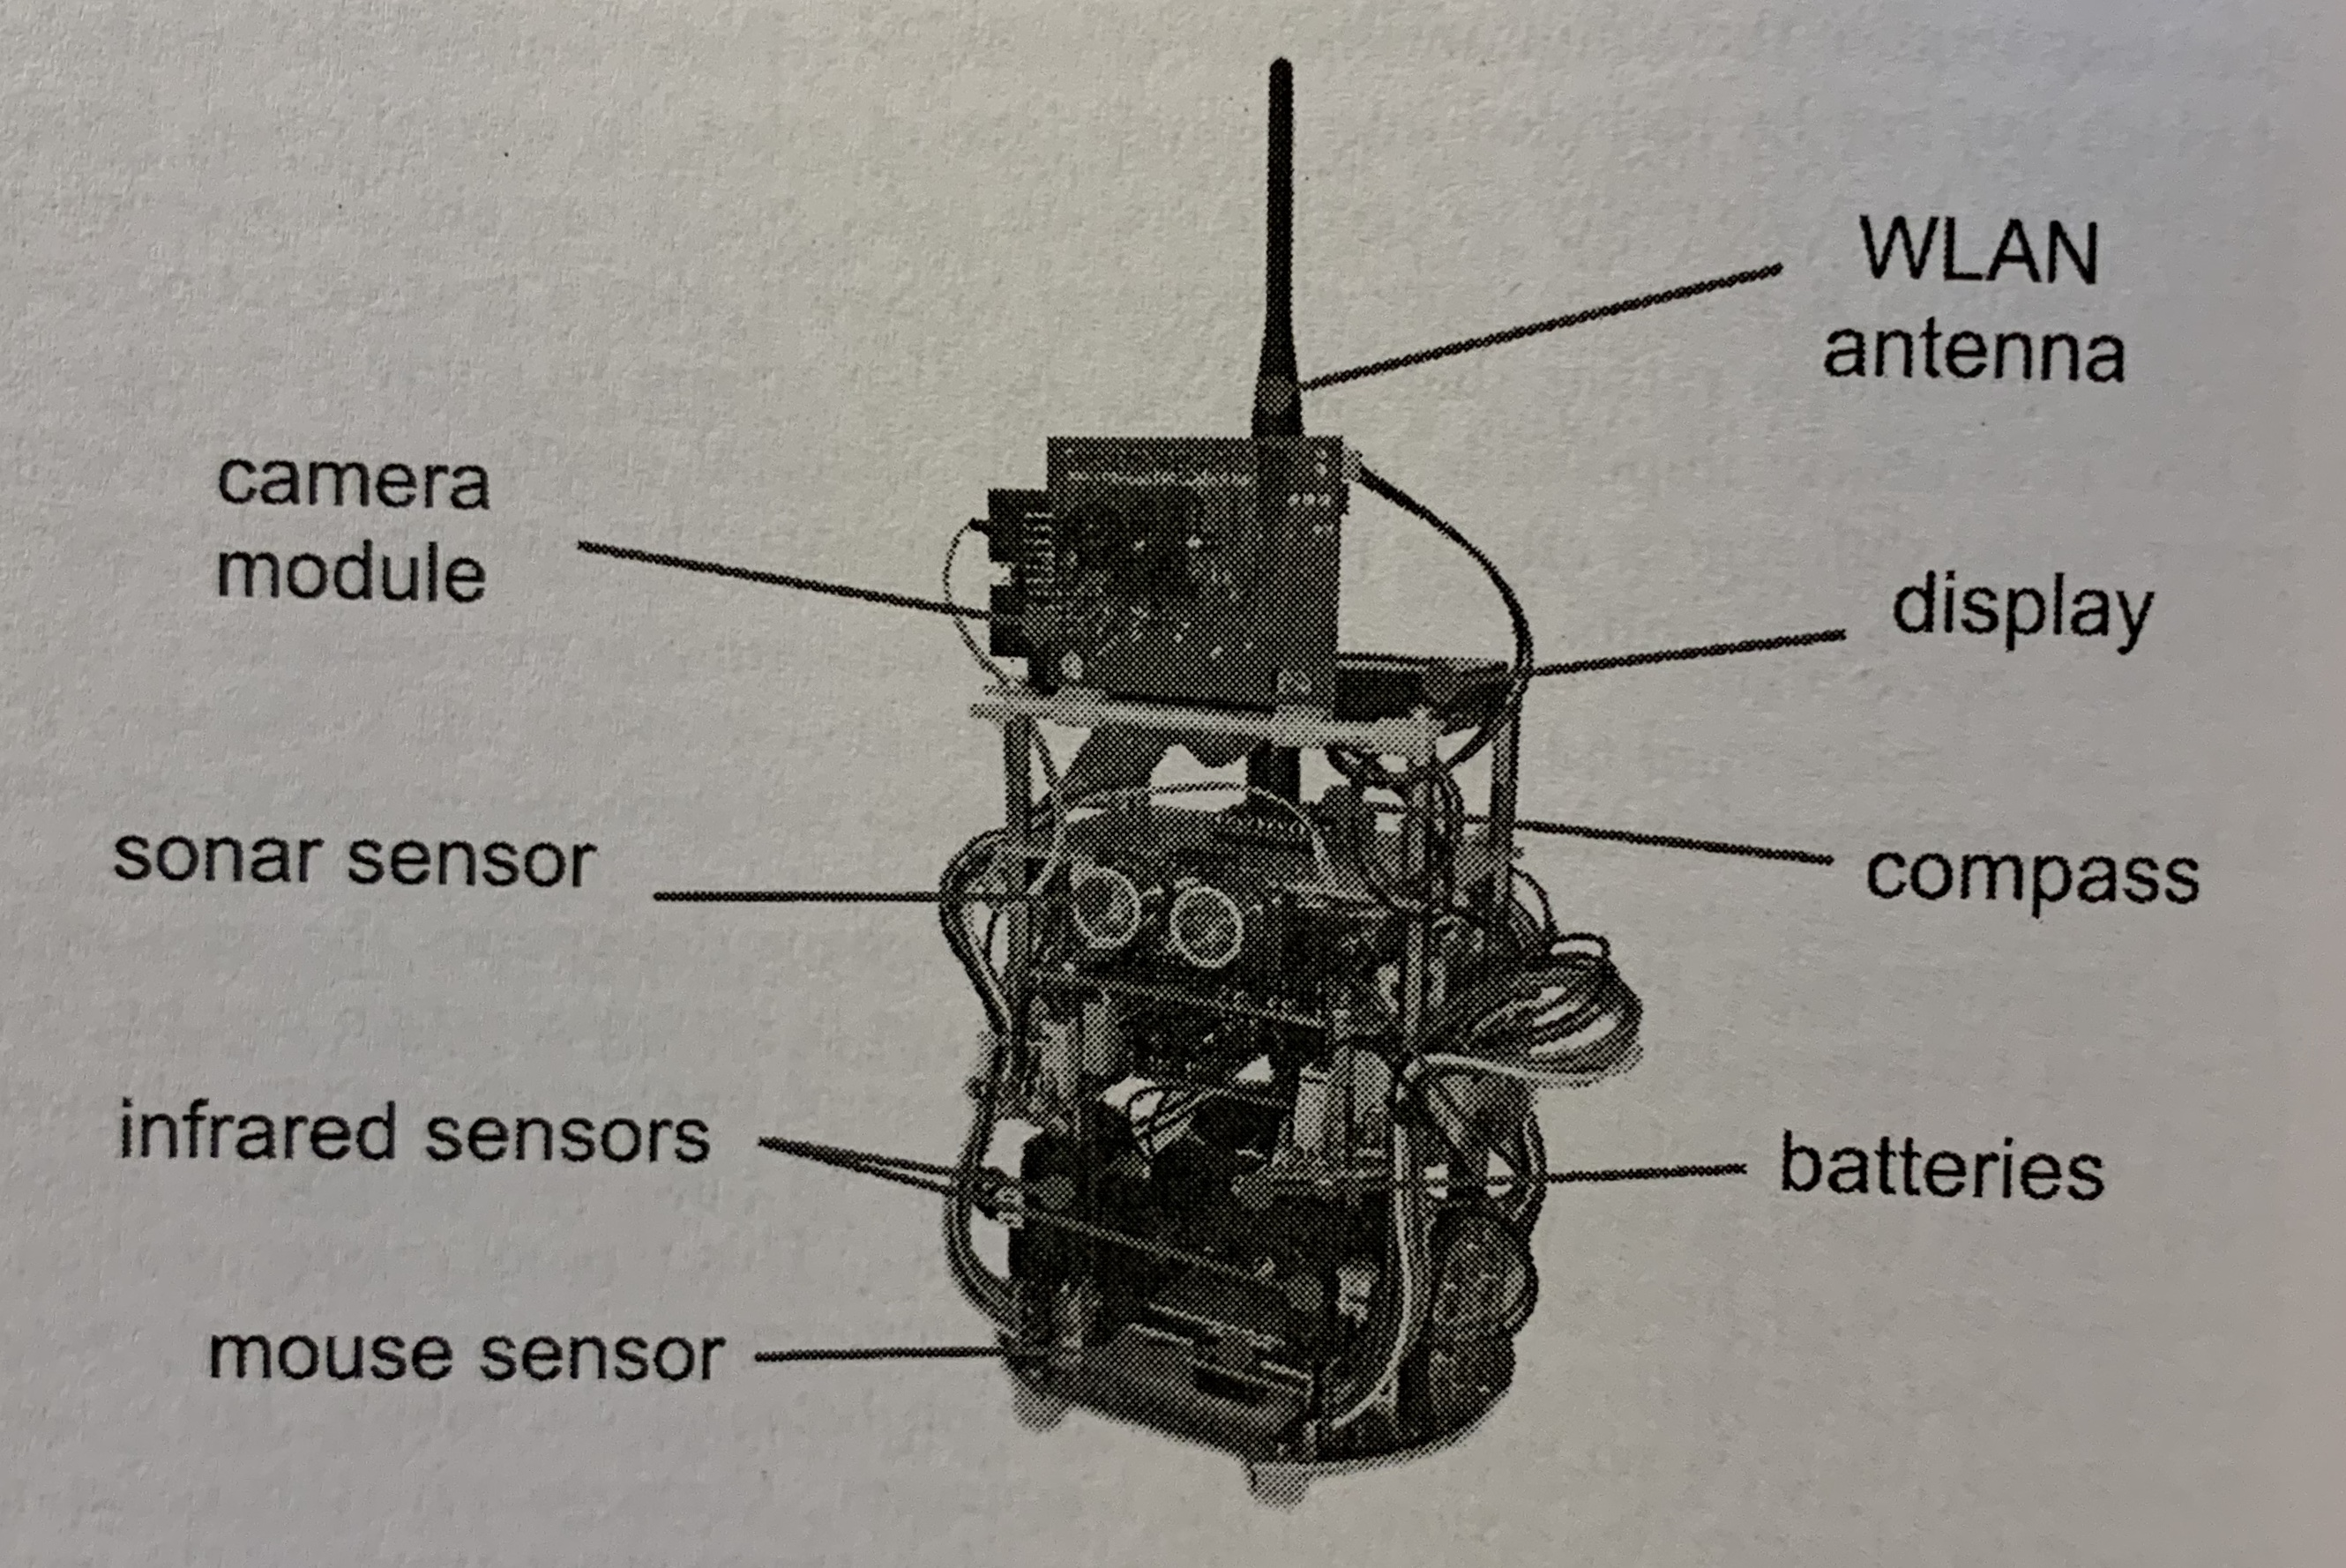
\includegraphics[scale=0.1]{images/CBot_mod.jpg}
		\caption{Mainboard}
	\end{figure}
	
	Die übergebene Hardware wurde auf Funktionsfähigkeit überprüft und zukünftige Einsatzfähigkeit analysiert. 
	
	\subsubsection{Hauptplatine}
	Die erste Generation des Ct'Bot wurde mit einem Atmel ATmega32 bestückt. Dieser konnte jedoch zu einem ATmega644 erweitert werden, wie es auch bei dem vorliegenden Ct'Bot der Fall ist. Der ATmega 644 arbeitet dabei mit 24 MHZ, 4kB Ram und 64kB Flash Speicher. Verbaut war der Hauptprozessor auf der mittleren Platine. Dieses wurde oft Mainboard genannt, da es die komplette Sensorik bündelte und die einzige, standartmäßig verbaute Platine war. 
	
	\begin{figure}[!htb]
		\centering
		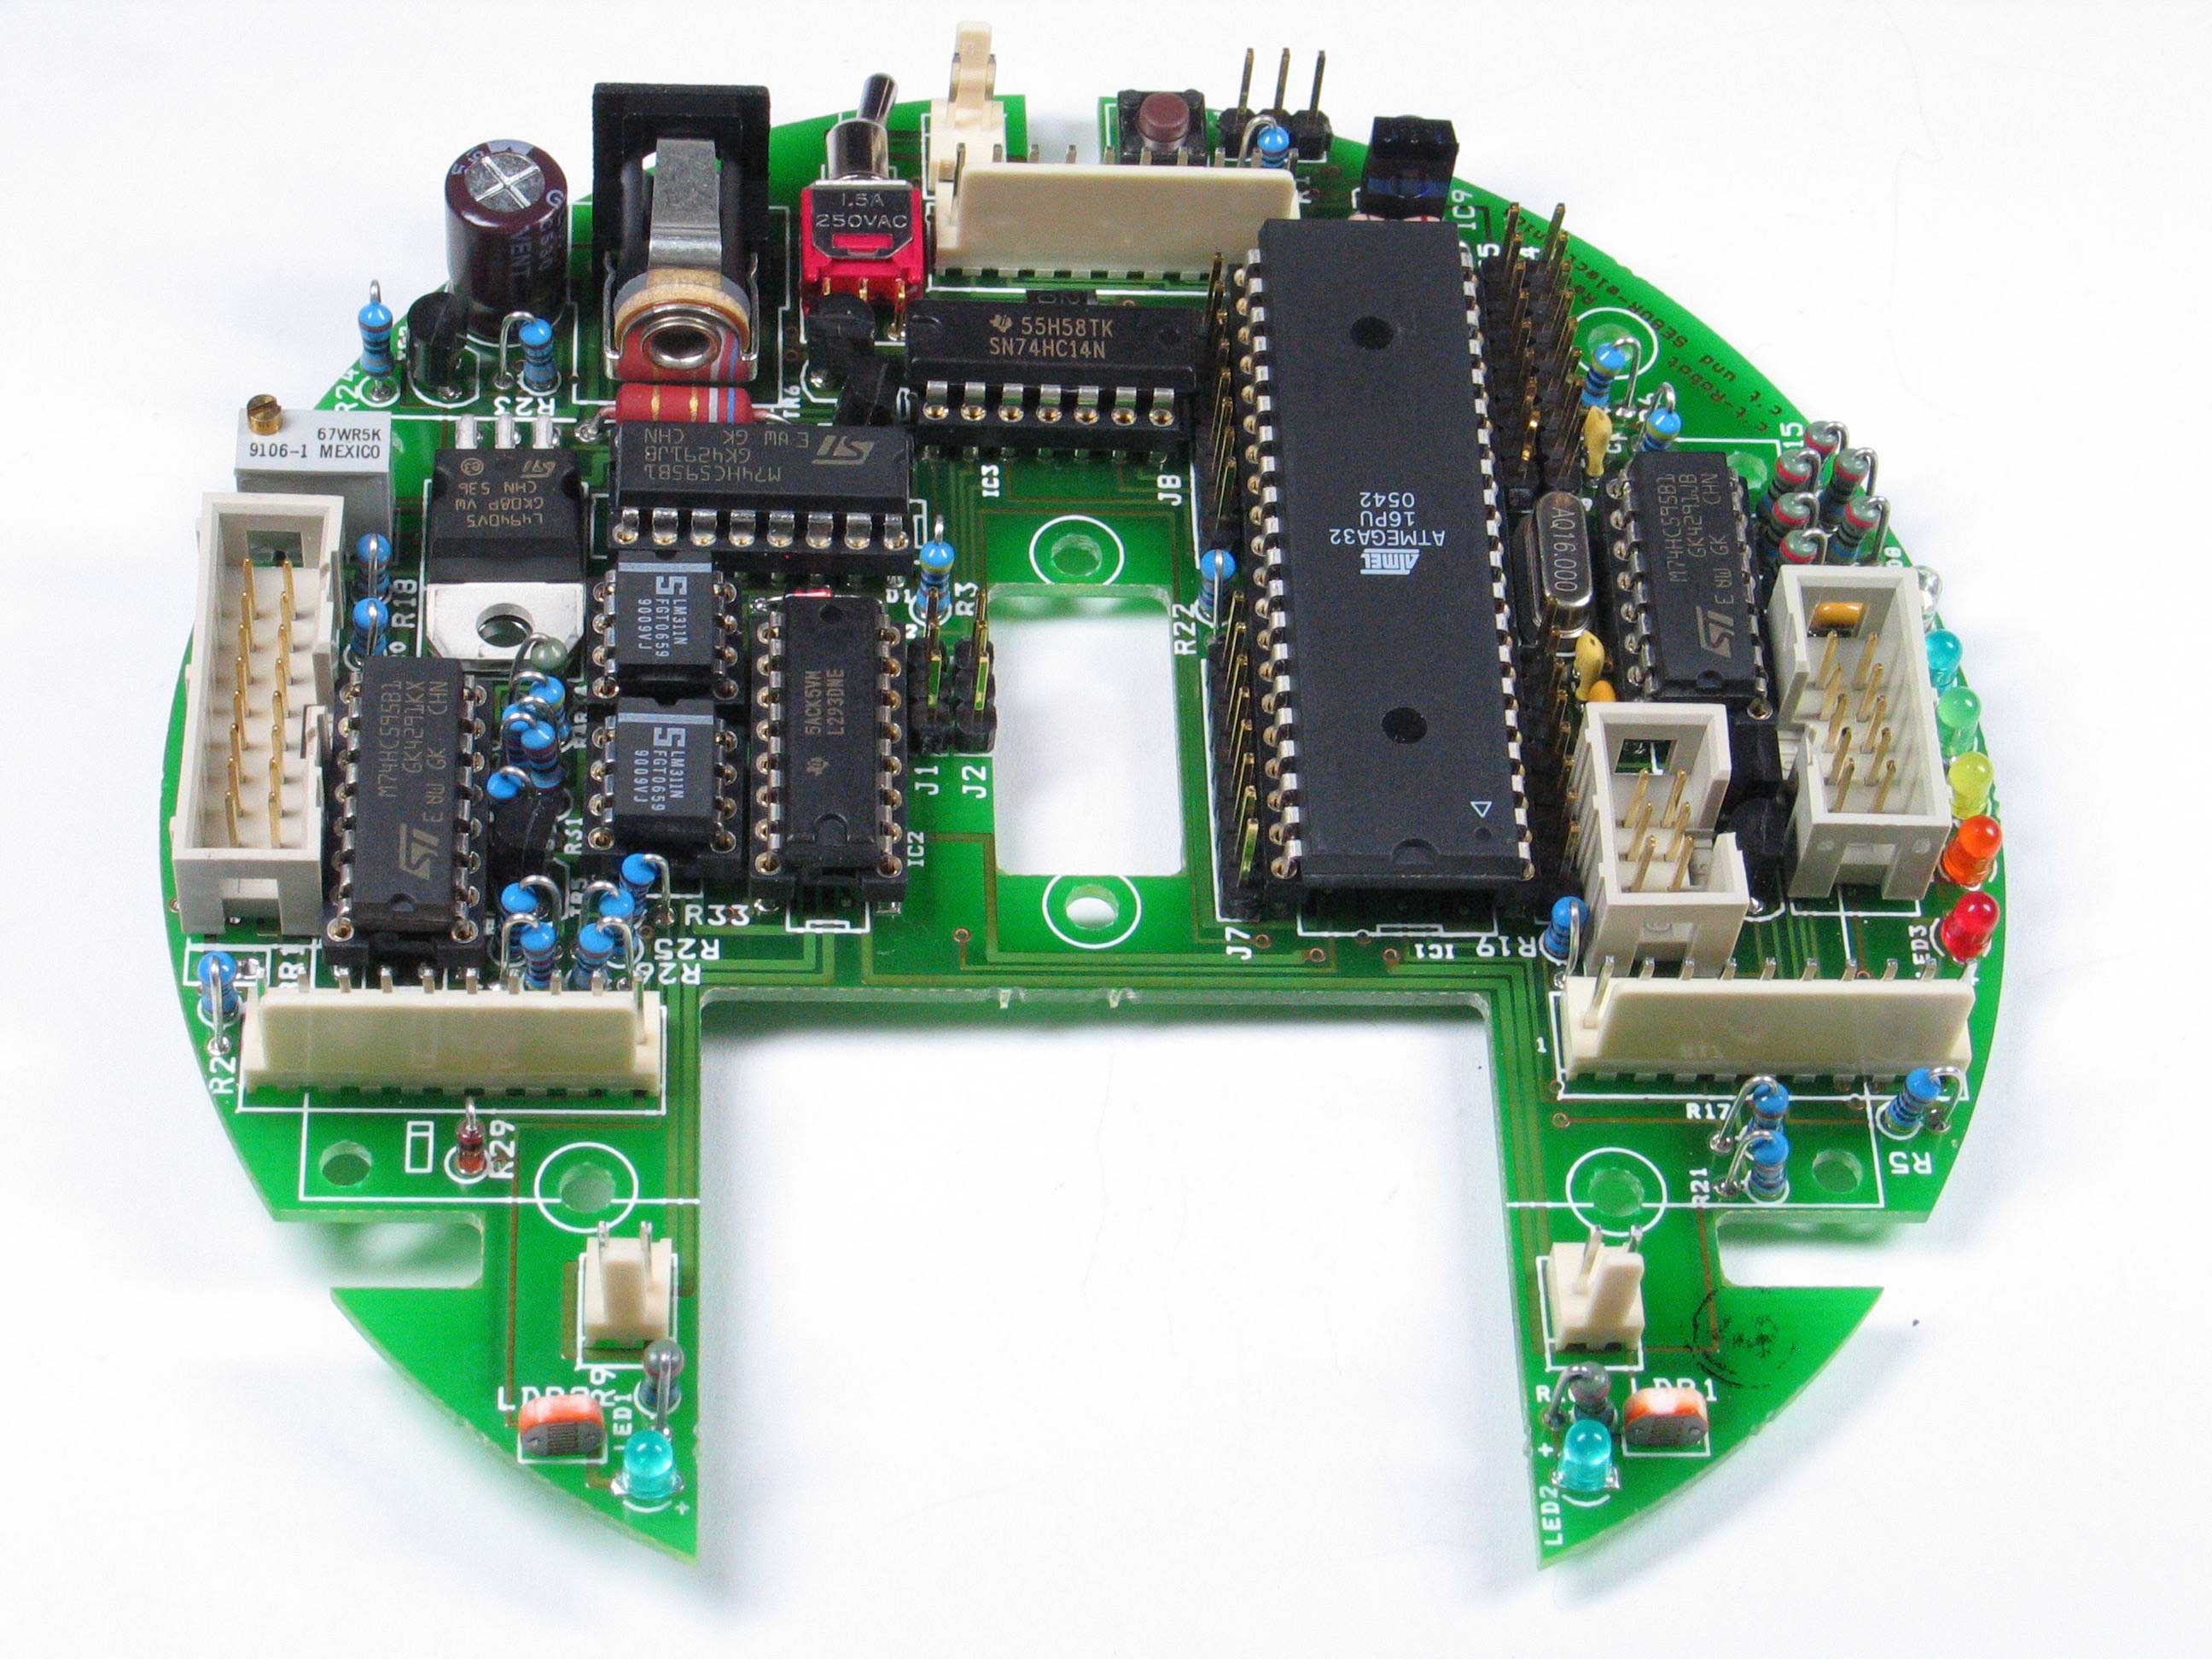
\includegraphics[scale=0.1]{images/mainboard.jpg}
		\caption{Mainboard}
	\end{figure}
	
	Die CPU war ausreichend um den Ct'Bot zu kontrollieren und einfache Aufgaben zu berechnen und auszuführen. Scheiterte jedoch an größeren Daten oder Karten wegen mangelnder Rechenleistung und Speicherplatz. 
	
	\subsubsection{Wheel-Encoder und Cliff-Detektoren}
	Als 'Lichtschranken' vermarktete CNY70 fungieren beim Ct-Bot als Wheel-Encoder und Cliff-Detektoren. Diese Sensoren können auf 1-2mm Distanz exakt hell-dunkel Übergänge auf einer Fläche erkennen. Dabei produzieren Sie ein analoges Ausgangssignal, welches ansteigt auf dunklen Flächen und wieder abnimmt auf helleren. Diese Eigenschaft wird gepaart mit einer Kodierungsscheibe um die Radachse herum. Diese besteht aus eng beieinander liegenden Schwarz-Weiß-Balken. Richtet man den CNY70 danach aus, so erkennt er - bei Bewegung des Rads und der Kodierungsscheibe - die Wechsel. Diese nennt man Ticks. Ein guter Tick-Wert für ein Rad mit 3cm Durchmesser wären 200-300 Ticks. Der Ct'Bot hat 64. Diese werden mit dem CNY70 in der vorgegebenen Konstruktion kaum erreicht, da der Sensor sehr empfindlich auf Umgebungslicht reagiert und zu weit vom Rad entfernt sitzt. \\
	Das gleiche Problem ergibt sich bei den Cliff-Detektoren. Das sind CNY70-Sensoren an der vorderen Roboterseite. Sie blicken Richtung Boden und sollen erkennen, wenn der Roboter sich über einem Abgrund befindet. In diesem Fall schalten sie ebenso ein analoges Output-Signal hoch. Leider waren die Sensoren zu hoch angebracht und lieferten daher fehlerhafte Werte. 
	
	\subsubsection{Motor}
	Der Ct'-Bot wird von 2 Faulhaber 2619 SR 006 DC-Motoren bewegt. Sie werden mit 5 V betreiben. 
	
	\subsubsection{Distanzsensoren}
	Als Distanzsensoren dienen zwei Infrarot-Distanzsensoren GP2D12 von Sharp. Diese haben einen Messbereich von 10-80cm und arbeiten mit Infrarot-Strahlen. Dies ermöglicht eine Punktgenaue Messung mit zuverlässigen Werten. Jedoch sind die Sensoren anfällig gegenüber Materialoberflächen. So können gemessene Daten stark voneinander abweichen, je nachdem auf welche Fläche sie treffen. Ebenso von Nachteil ist der hohe Stromverbrauch und die fehlende Abschirmung der Sensoren. Ihre Platine ist ungeschützt und frei liegen zur Rückseite. \\
	Der auf dem Bild dargestellte Sonar-Sensor wurde nicht mehr aufgefunden und wird daher nicht als vorhandene Sensorik geführt. 
	
	\subsubsection{Kompass}
	Für die Messung der Ausrichtung wurde dem Ct'Bot nachträglich ein Kompass von Devantech installiert. Der CMPS03 hat eine Genauigkeit von 3-5 Grad und misst in Bezug zum Nordpol. Die exakte Kalibrierung des Kompass ist äußert mühsam und wurde von \cite{Hofmeister} in seiner Doktorarbeit beschrieben. Ebenso hatte dieser wiederholt Probleme mit der Genauigkeit der Messungen. 
	
	\subsubsection{Optical-Flow Sensor}
	\begin{figure}[!htb]
		\centering
		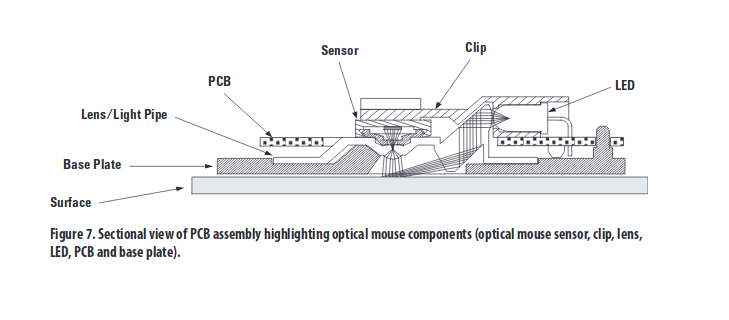
\includegraphics[scale=0.55]{images/adns.png}
		\caption{ADNS 2610 Skizze aus dem Datasheet}
	\end{figure}
	Als weitere Odometrie-Sensor hat der Ct'Bot einen ADNS-2610 Optical-Flow-Sensor von Avago verbaut. Der Optical-Flow-Sensor ist im hinteren Teil des Roboters angeschraubt und in der Werksausführung zu weit vom Boden entfernt, so dass er keine korrekten Werte liefert. Wird der Sensor tiefergelegt, so misst er den Fluss von Pixeln in schnell hintereinander aufgenommen Bildern und berechnet daraus eine Veränderung der Lage. Dies funktioniert mit einer Auflösung von 0,635 mm (400 Counts Per Inch, CPI) \footnote{Siehe hierzu Datenblatt des Sensors}. Somit sehr exakt. 
	
	\subsubsection{LCD}
	Es wurde zusätzlich ein DEM20485 LCD von Ryston verbaut. Leider war dieser nicht mehr ganz funktionstüchtig. Es existierte ein Fehler, welcher die Darstellung von Charaktern im unteren Feld nicht ermöglichte. 
	
	\subsubsection{Kamera}
	Der Ct'Bot verfügte über ein Kamera-Modul. Diese konnte Bilder in der Auflösung von ... erstellen. Leider ist der Speicherplatz des Ct'bot hierfür nicht ausreichend, daher musste eine zusätzliche SD-Karte eingebaut werden. Diese war ebenfalls nicht vom Ct'bot direkt lesbar. Er konnte nur Speicher- und Sendebefehle ausführen, jedoch nicht darstellen oder analysieren. 
	
	\subsubsection{verschiedene Chips}
	Ein zusätzliches Wlan-Modul von Lantronic ermöglichte die Kommunikation mehrerer Ct'Bots miteinander. Die Funktionstüchtigkeit des Moduls konnte nicht überprüft werden. \\
	Das SD-Karten-System ist ein selbst entwickeltes Modul und kann 512 Byte pro 5ms (also 0,5MB/s, die Raspberry Pi 3 hat im Vergleich eine durchschnittliche Schreibgeschwindigkeit von 20-50MB/s, abhängig von eingesetzter Karte, eine moderne SSD etwa 500-3500MB/s) schreiben. Beim Schreiben und Lesen wird auf der Karte kein Fat32 Format verwendet, sondern ein selbstgeschriebenes Format genutzt. Dies verzichtet auf einen spezielles Dateisystem und nummeriert die Blöcke durch. Diese werden nun von vorne beginnend geschrieben. Ein Zugriff beginnt daher immer am ersten Block und iteriert bis zur gesuchten Nummer durch die ganze Karte. Große Karten verzögern daher den Zugriff enorm. Ein praktischer Nutzen für moderne Systeme ist dadurch nicht mehr gegeben. 
	
	\subsubsection{Grundplatte}
	Eine Aluminium-Platte mit einem Durchmesser von 12 Zentimetern bildet die Grundplatte. Der ganze Ct'Bot ist so konzipiert, dass diese Grundplatte modular Erweitert werden kann. Jedes neue Modul wird hierbei auf die bisher oberste Platte aufgeschraubt. Dadurch wächst der Roboter in die Höhe und behält seine Grundform bei. Immer dabei war die erste Ebene, das Mainboard. Alle weiteren Erweiterungen waren spezielle Zukaufteile oder selbst entwickelt. 
	
	\subsubsection{Fehlende Bauteile}
	Nicht mehr vorhanden waren das Batteriefach, ein PC-Kabel (9-Poliger D-Sub-Stecker, leider kein Anschluss an moderne Rechner möglich da dies ein überholtes Format ist), die Fernbedienung und der Ultraschall-Distanzsensor. 
	
	\subsection{Neue Hardware}
	In diesem Abschnitt wird die neue Hardware vorgestellt mit einer kurzen Begründung warum diese ausgewählt wurde. 
	
	\begin{figure}
		\centering
		\subfloat[Seitenansicht rechts]{{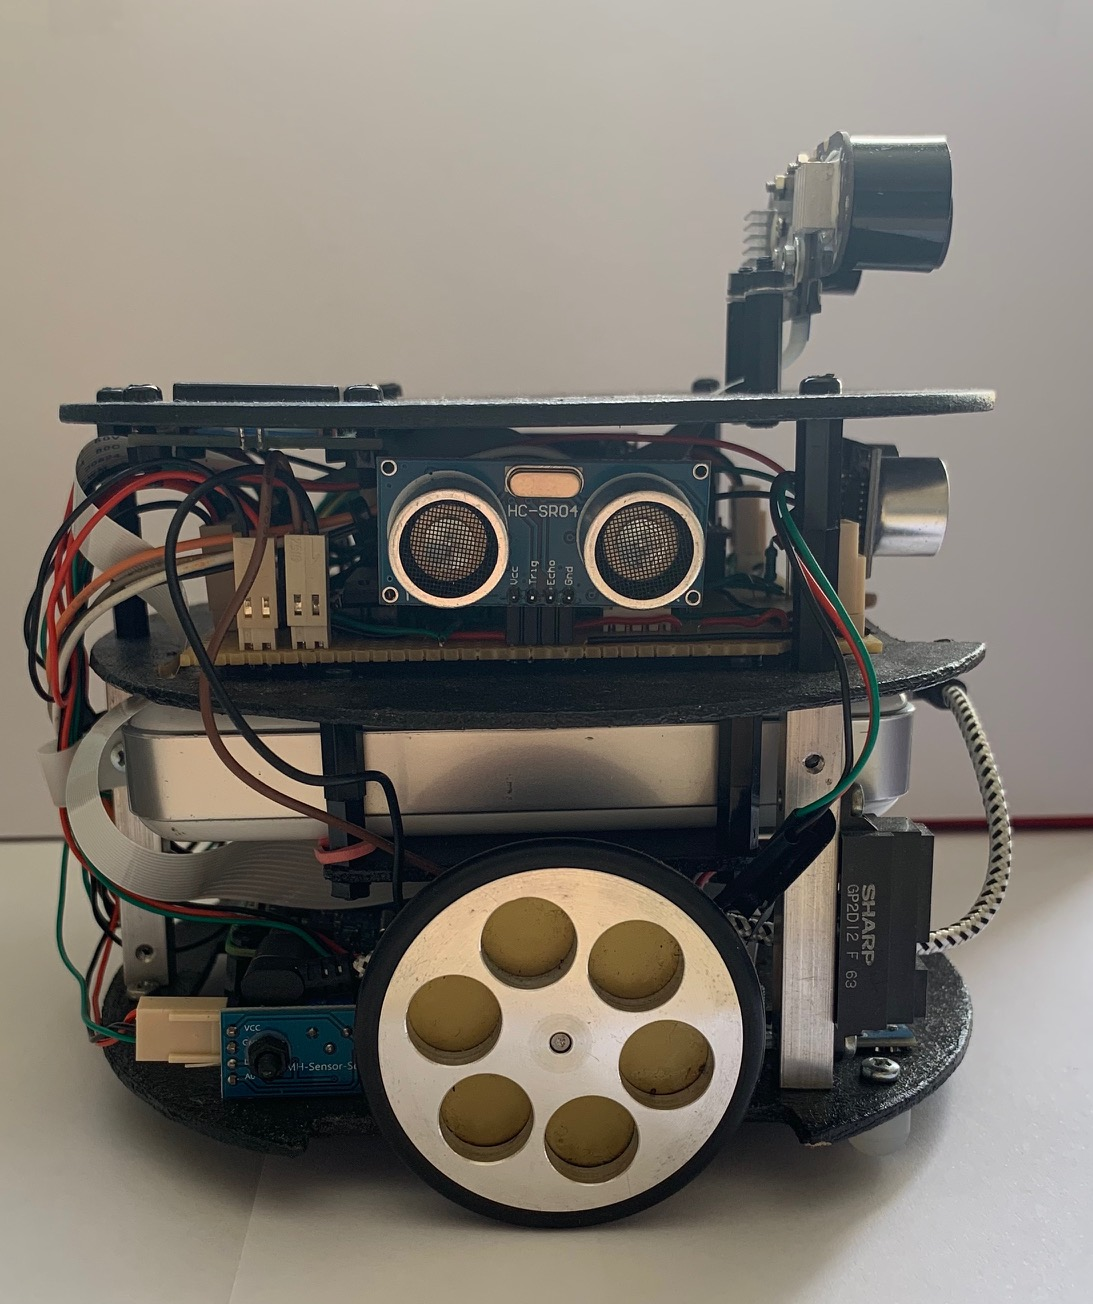
\includegraphics[width=5cm]{images/pybot_rechts.jpg} }}%
		\qquad
		\subfloat[Frontansicht]{{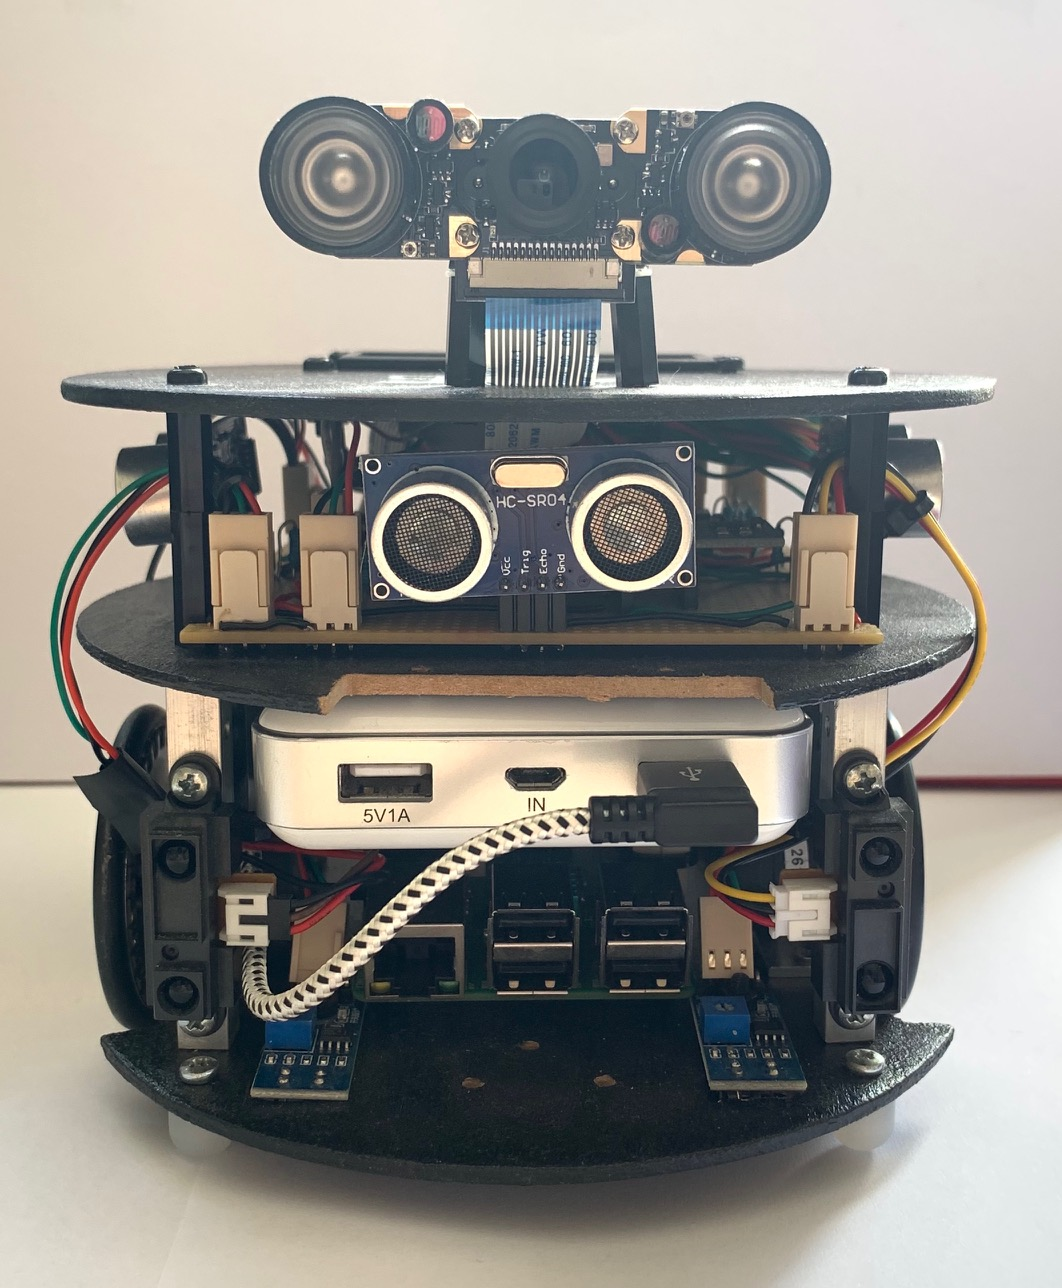
\includegraphics[width=5cm]{images/pybot_vorne.jpg} }}%
		\qquad
		\subfloat[Seitenansicht links]{{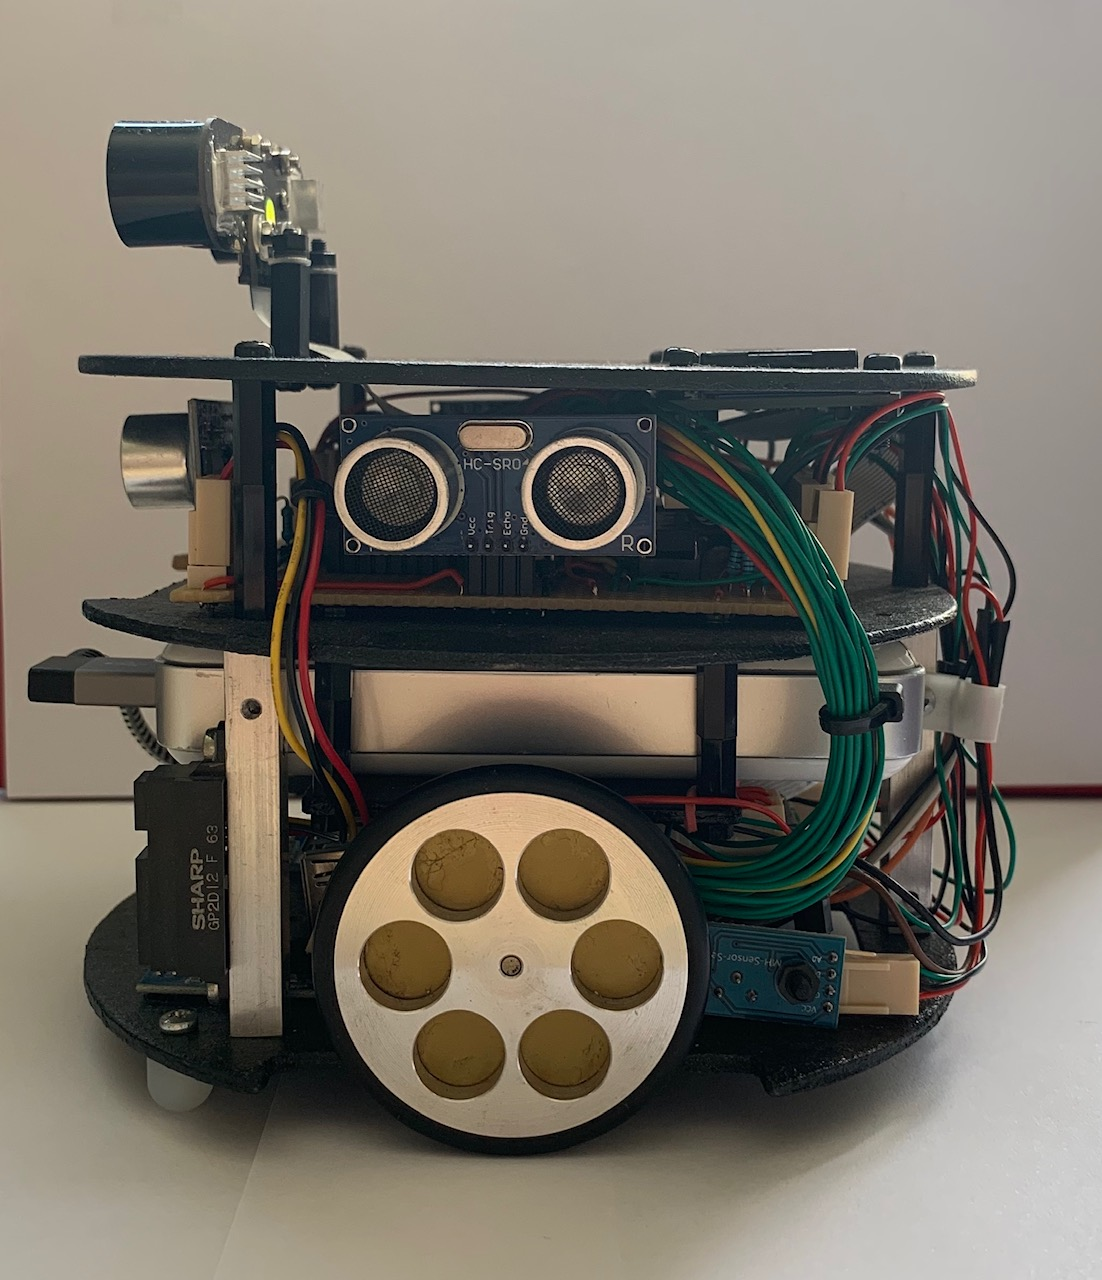
\includegraphics[width=5cm]{images/pybot_links.jpg} }}%
		\qquad
		\subfloat[Rückseite]{{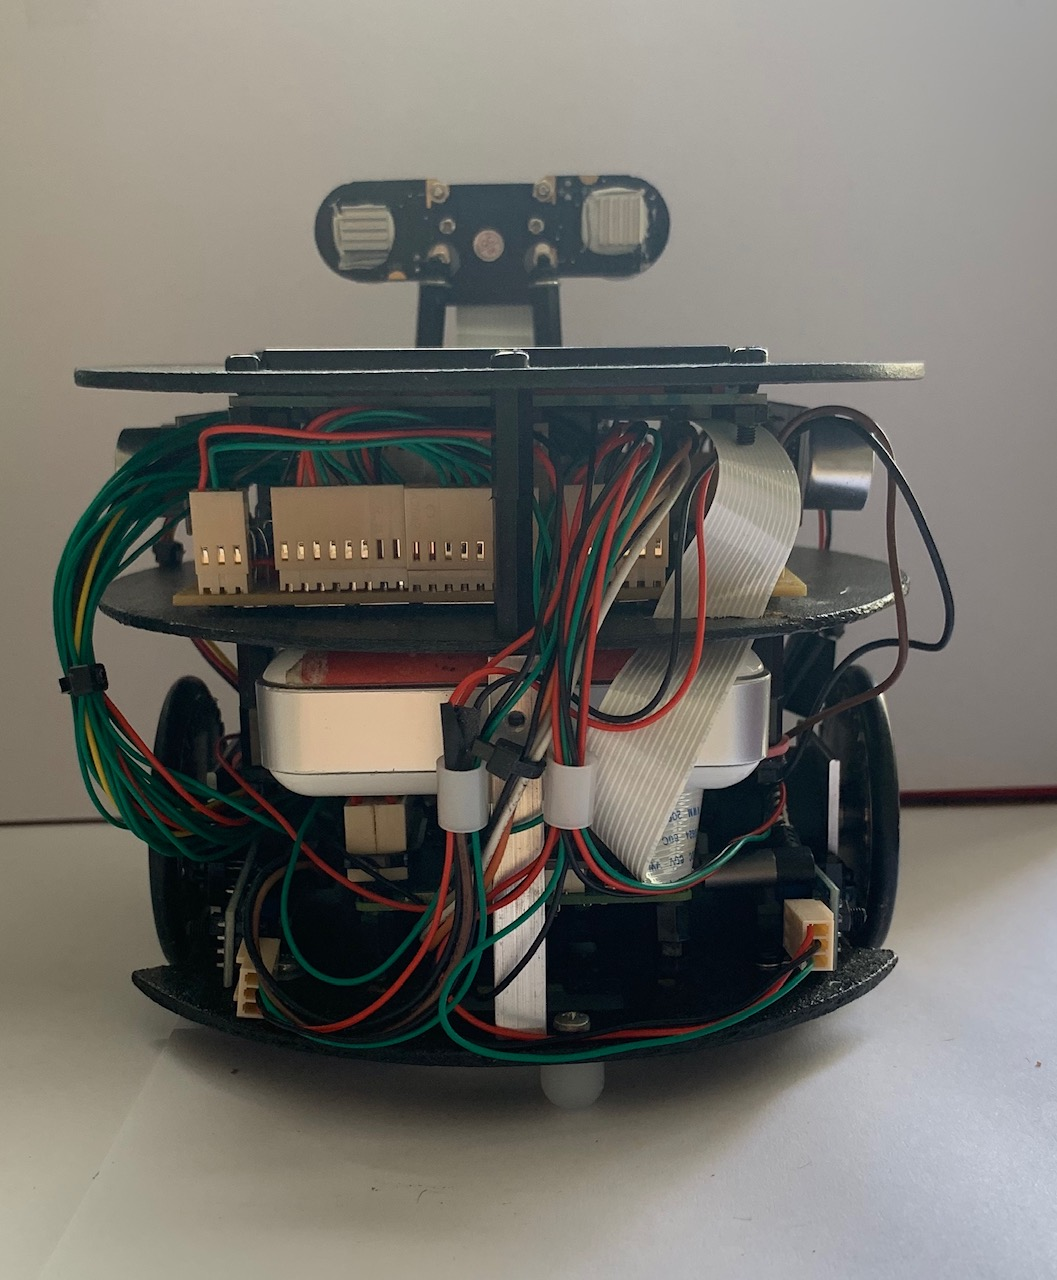
\includegraphics[width=5cm]{images/pybot_hinten.jpg} }}%
		\caption{Der fertige PyBot}%
		\label{fig:example}%
	\end{figure}
	
	
	
	
	\subsubsection{Hauptplatine}
	Der bisherige CPU wird für die künftigen Aufgaben nicht leistungsstark genug sein. Als Alternative würde sich erneut ein ATmega anbieten, wie z.B. der ATmega328P. Dieser ist auf dem Arduino Uno verbaut und kostet als Einplatinen-Computer 20Euro. Er bietet die Möglichkeit digitale und analoge Pins anzusteuern und hat eine ausreichend starke Rechenleistung. Jedoch ist hier, ebenso wie bisher, der Speicherplatz mit 32kB begrenzt. Für komplexere Projekte empfiehlt sich daher eine Raspberry Pi 3B. Mit einem Preis von ca. 35 Euro ist sie zwar teurer, erlaubt aber den Speicherplatz variable zu vergrößern. Zusätzlich ist sie - in Verbindung mit Raspbian - ein vollständiger Stand-alone-PC und erlaubt so die Verwirklichung von hochkomplexen Steuerungen oder Algorithmen. Ein weiterer Vorteil ist ihre kompakte Größe, ihre leichte Programmierbarkeit und der niedrige Stromverbrauch. \\
	Die Pi hat den Nachteil, dass sie keine analogen Eingänge besitzt. Dies muss über einen  Analog-Digital-Konverter (ADC) kompensiert werden. \\
	Weitere Möglichkeiten wären ein Asus Tinker Board, Banana Pi, BeagleBoard oder HumminBoard. Diese bieten meist gleiche bis etwas mehr Ausstattungsmerkmale als die Pi, kosten jedoch bis zu drei Mal soviel. 
	
	\begin{figure}[!htb]
		\centering
		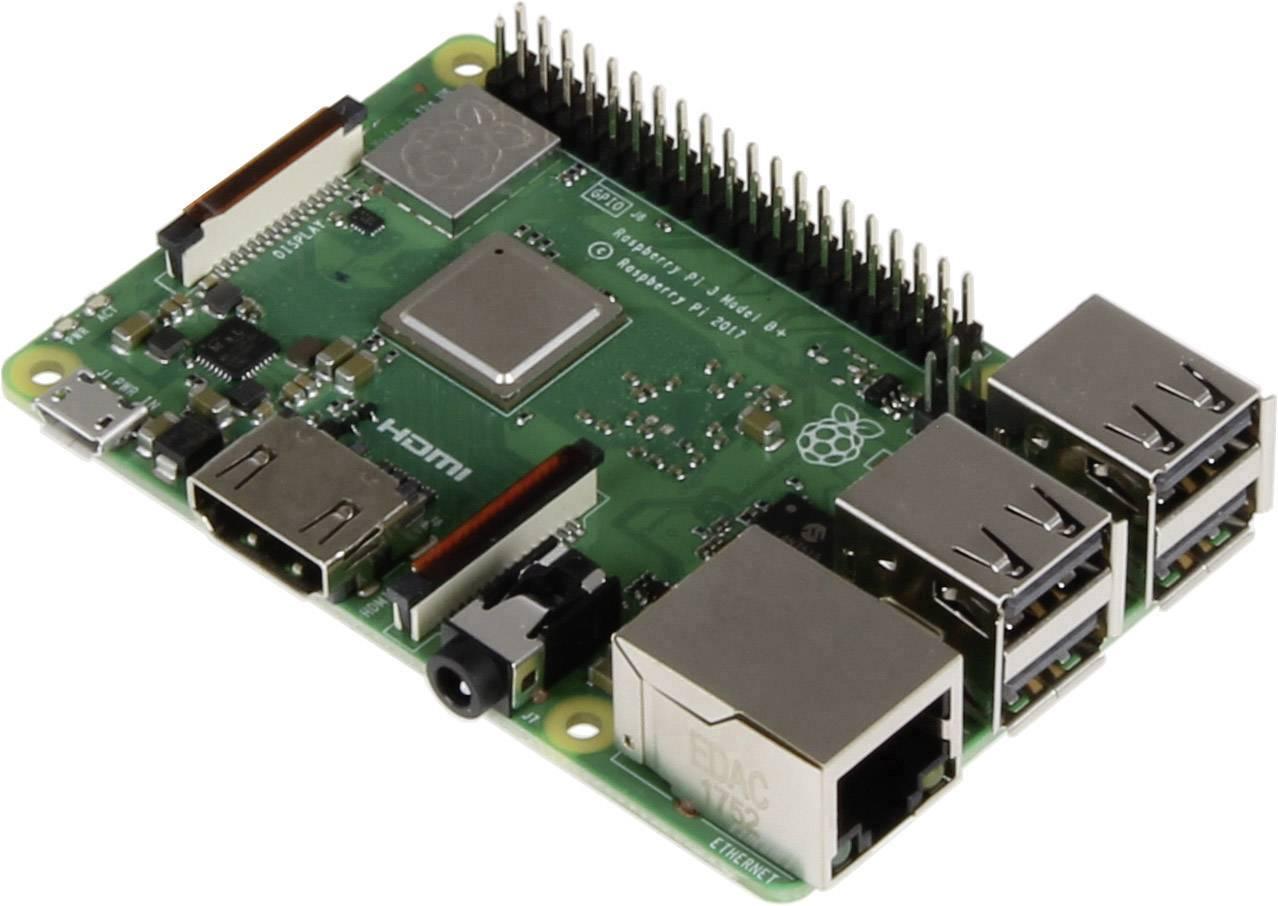
\includegraphics[scale=0.25]{images/Pi.jpg}
		\caption{Raspberry Pi - offizielles Bild des Herstellers}
	\end{figure}
	
	Die Raspberry Pi 3B+ hat einen Broadcom Chip mit 1.4Ghz, 1GB SDRAM, eingebautes Wlan und Bluetooth, ein Ethernet-Stecker, 4 USB-Ports, einen Stecker für eine Kamera, HDMI-Ausgang, einen Micro-SD Steckplatz und 40 programmierbare Pins für digitale In- und Outputs. Sie wird mit 5V betrieben. \footnote{Daten aus dem Datenhandbuch, Bild von der Offiziellen Website}\\
	Diese Spezifikationen sollten für unsere Software-Anforderungen ausreichen. 
	
	\subsubsection{Kamera}
	
	\begin{figure}[!htb]
		\centering
		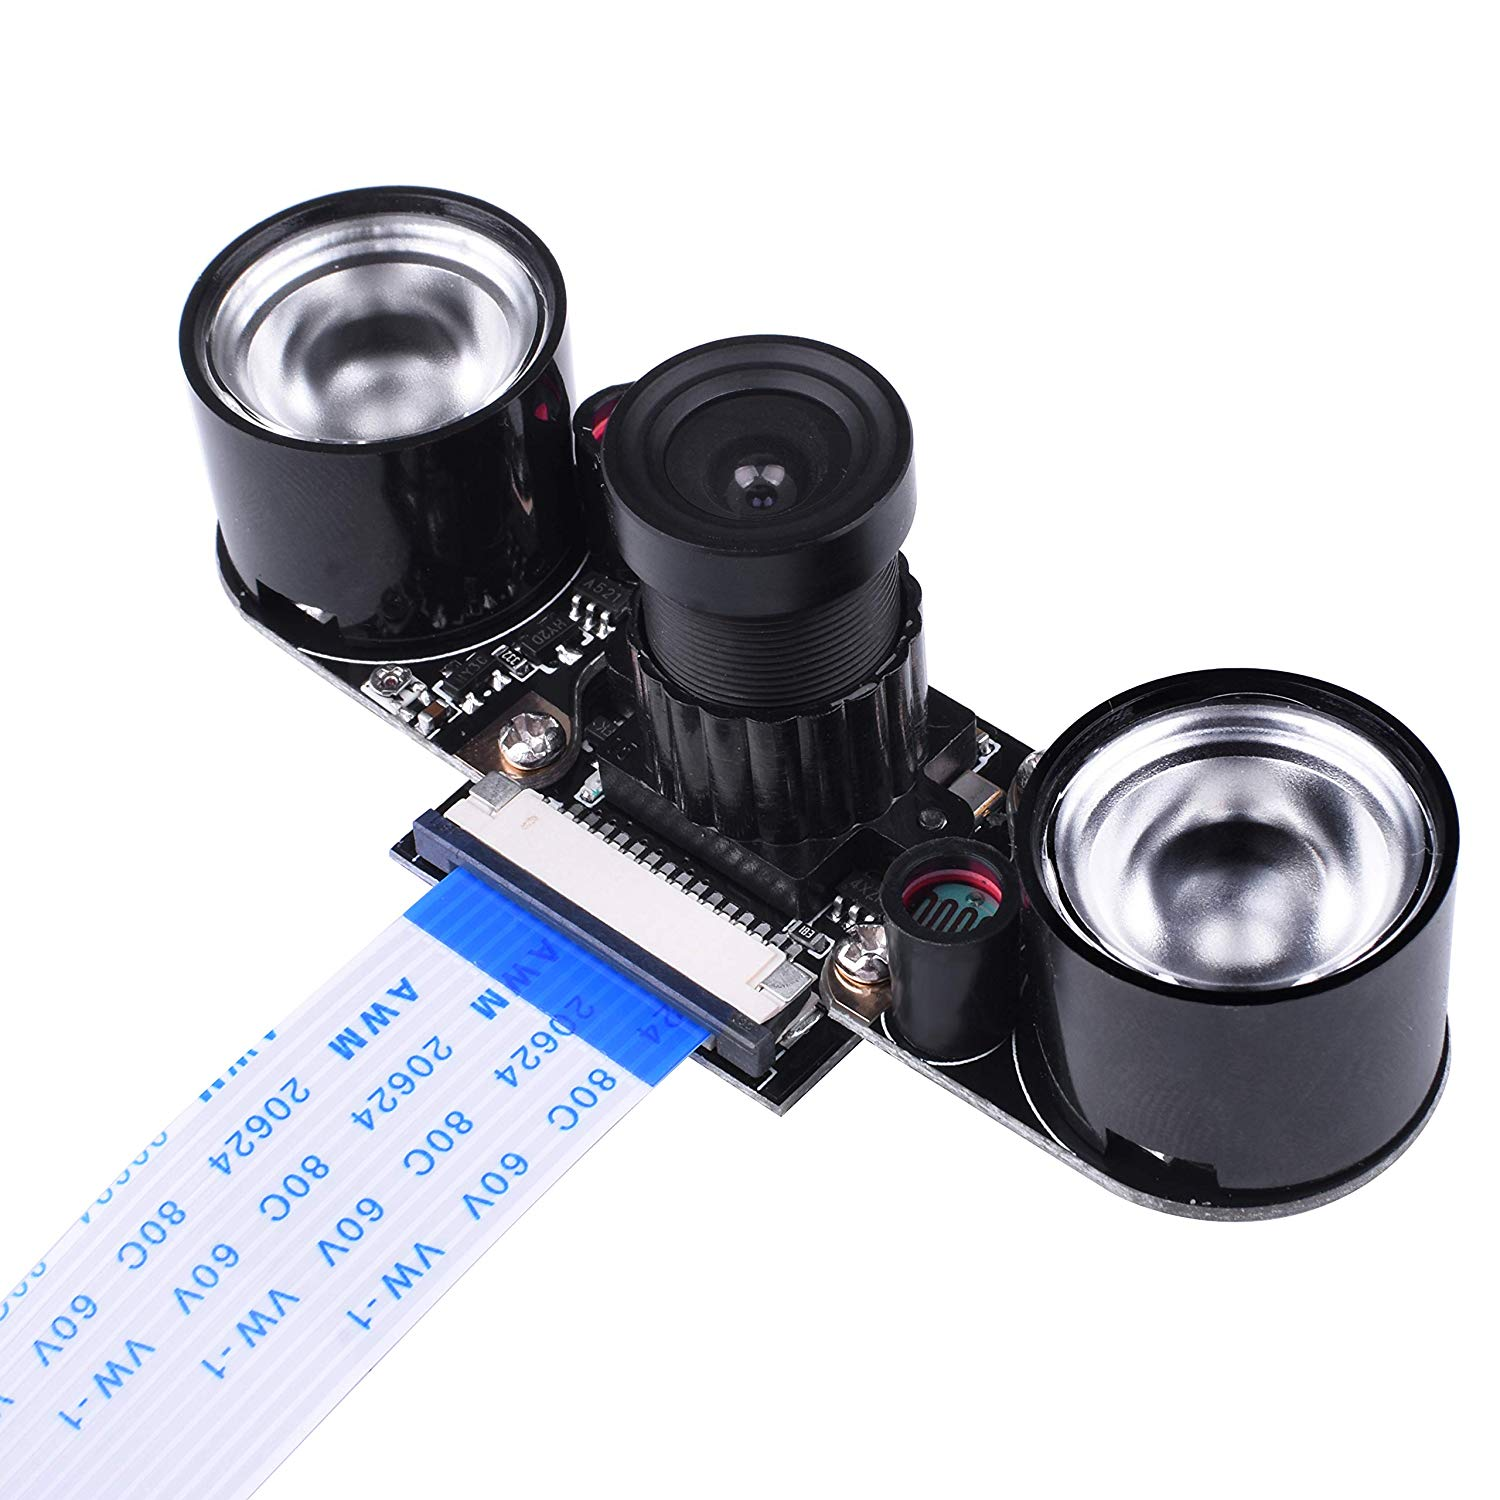
\includegraphics[scale=0.1]{images/Kuman_Kamera.jpg}
		\caption{Raspberry Pi Nachtsichtkamera der Firma Kuman - offizielles Bild des Herstellers}
	\end{figure}
	
	Die bisherige Kamera lässt sich nicht an die Pi anschließen. Daher wird Sie durch eine Raspberry-Pi Kamera ersetzt. Hierbei wird nicht die übliche Ausführung gewählt, sondern eine mit kontrollierbarem Infrarot-Filter. Durch diese Option ist es der Kamera möglich auch in völliger Dunkelheit Bilder aufzunehmen. Die Kamera der Firma Kuman hat eine Auflösung von $2592 \times 1944$ und einen manuell verstellbaren Fokus. Dies senkt die Kosten, muss aber bei der Einstellung mit bedacht werden. Weiterhin hat sie seitliche Infrarot-LEDs um den Infrarot-Filter bei Tageslicht zu kompensieren. Ohne diese LEDs würden die Bilder der Kamera in einer hellen Umgebung einen sehr hohen Anteil an rot-Werten aufweisen, welche eine übliche Kamera nicht hätte. Dies muss bei einer weiteren Bildverarbeitung mit eingeplant werden, da trotz der LEDs die Bilder erhöhte rot-Werte enthalten. 
	
	\subsubsection{Akku}
	Der Ct'Bot wurde von einem Akku-Pack betrieben, welcher aus zusammengeschlossenen AA-Batterien bestand. Hiervon waren 6 nötig. Dies begrenzte die Flexibilität und wird daher durch eine handelsübliche Powerbank ersetzt. Diese sollte mindestens 10.000mA haben um eine Laufzeit von mindestens 6 Stunden zu gewährleisten \footnote{diese Zeitangabe bezieht sich auf aktive 6 Stunden Fahren und Applikationsausführung, inklusive eines Video- und VNC-Streams}. Weiterhin ist darauf zu achten, dass sie über ein USB-Kabel angeschlossen werden kann. 
	
	\subsubsection{Wheel-Encoder}
	Die bisherigen Wheel-Encoder waren unzuverlässig. Ihre Fehlerquote an verpassten Räder-Ticks war nicht korrekt messbar, da Sie von 64 Ticks höchstens die Hälfte erkannten und somit ein korrekter Ablauf kaum möglich war. Sie wurden durch eine verbesserte Variante des CNY70 ersetzt. Die neuen Wheel-Encoder sind TCRT5000 Chips. Ihr Messprinzip ist analog zum CNY70. Verbessert sind jedoch die Reaktion auf einen Input, das Hinzufügen eines digitalen Ausgangs, die absolute Distanz auf die gemessen werden kann wurde auf 2cm erhöht und eine Regulierbarkeit der Jump-Spannung ist nun gegeben, d.h. der benötigte Hell-Dunkel-Unterschied der Übergänge kann manuell eingestellt werden. Die neuen Sensoren erkennen nun zuverlässig die Räder-Ticks, leiden aber weiterhin an den grundsätzlichen Problemen der Rad-Odometrie. 
	
	\subsubsection{Distanzsensoren}
	Die GP2D12 werden heute noch in neuere Systeme verbaut. Es besteht kein Grund diese Auszutauschen. \\
	
	\begin{figure}[!htb]
		\centering
		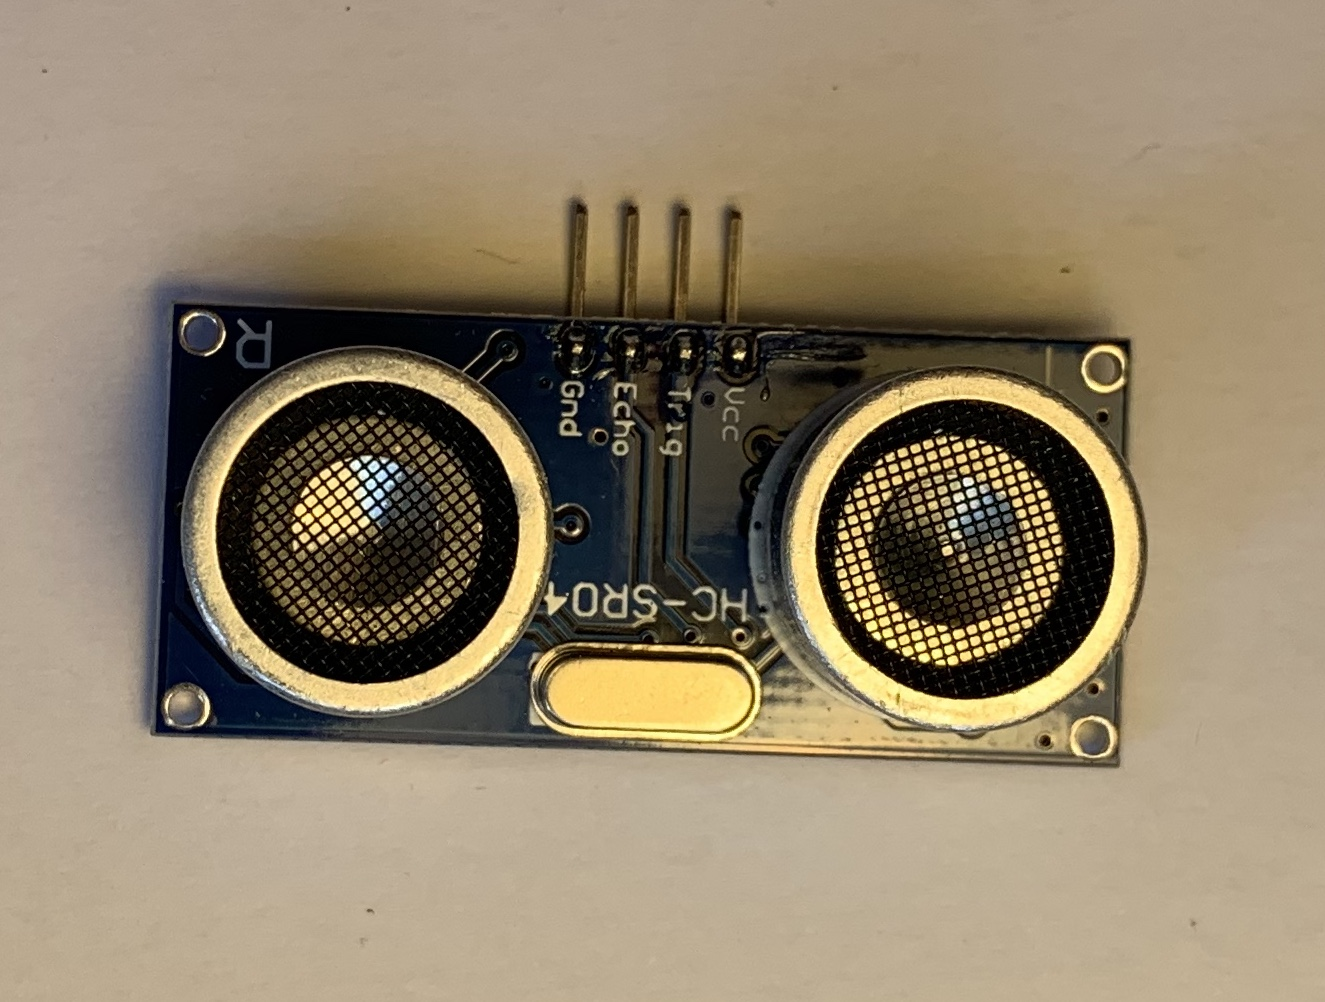
\includegraphics[scale=0.1, angle=180]{images/ultraschall2.jpg}
		\caption{Ultraschall-Sensor HC-SR04}
	\end{figure}
	
	Der Roboter wird jedoch um Ultraschall-Distanz-Sensoren erweitert. Diese erlauben eine Abschätzung der Distanz auf 10-60cm. Zu beachten ist, dass die Ultraschall-Distanz-Sensoren einen breiten Streubereich haben, welcher sich Kegelförmig vom Sensor im Raum ausbreitet. Während die Sharp-Sensoren punktgenau messen, misst ein Ultraschallsensor eine ganze Fläche ab und erhält dabei stets die kleinste gemessene Distanz.\\
	Weiterhin problematisch ist bei Ultraschall, dass die Sensoren miteinander interferieren können. Dies tritt insbesondere dann zu tage, wenn der Roboter sich auf engstem Raum bewegt. Daher dienen diese Sensoren tatsächlich nur der Abschätzung und um die bisher unerfassten Bereiche links und rechts vom Roboter zu messen. 
	
	\subsubsection{Gyroskop}
	Die Ungenauigkeit des Kompasses macht es nötig einen Ersatz zu suchen um die Ausrichtung des Roboters zu messen. Hierfür bieten sich kostengünstige MPU6050 Sensoren an. Diese können Drehungen und Beschleunigungen an der x-,y- und z- Achse bestimmen. Ihre Genauigkeit beträgt dabei 1-2 Grad für die Drehung. Sie verfügen über ein I2C-Kommunikations-Interface und können darüber an die Pi angeschlossen werden. 
	
	
	\subsubsection{Grundplatte}
	Die alte Grundplatte ermöglichte leider nicht den Einbau der Pi und der Powerbank in liegender Position. Daher wurde die Grundplatte von 12 auf 15cm Durchmesser erhöht. Dadurch war auch ein verbesserter Einbau der Cliff-Sensoren und des Optical-Flow-Sensors möglich. Dieser sitzt nun im Mittelpunkt auf der Grundplatte und macht dadurch eine Transformation seiner gemessenen Daten unnötig. Dies spart komplexe Matrix-Berechnungen in den x-y-Werten. 
	
	\subsubsection{Sensorplatine}
	Die Sensorplatte fasst alle Sensoren zusammen. Diese haben keinen Platz mehr auf dem Motherboard der Pi. Das alte Board konnte durch die Erweiterung nicht wiederverwendet werden. Daher wurde eine neue Sensorplatte entworfen und bildet nun die mittlere Schicht des Roboters. \\
	Grundlage der Sensorplatte ist eine 2.5-Punkt-Raster-Lötplatine. Auf dieser wurde der Schaltplan durch Kupferlitzen und Silber-Kupfer-Draht realisiert und die Sensorik über Pin-Stecker direkt auf der Platte installiert. Diese Lösung erlaubt einen schnellen Austausch von Sensoren und bietet eine Erweiterbarkeit auf die freien Pins an. Sensoren außerhalb der Platine wurden über Kupferlitzen und das PSK-Steckersystem eingebunden. Hierbei wurde ein einfacher Farbcode für die Leiter implementiert,so dass ein Tausch von Sensorik oder eine Fehlersuche im Kabelmanagment erleichtert wird. Für die Fehlersuche wurden zwei Zustands-LEDS verbaut. Dabei signalisiert die Grüne einen fehlerfreien Zustand und die rote LED leuchtet beim Aufruf jedes Python-Error-Exceptions. 
	
	\begin{figure}
		\centering
		\subfloat[Draufsicht auf die Sensorplatte]{{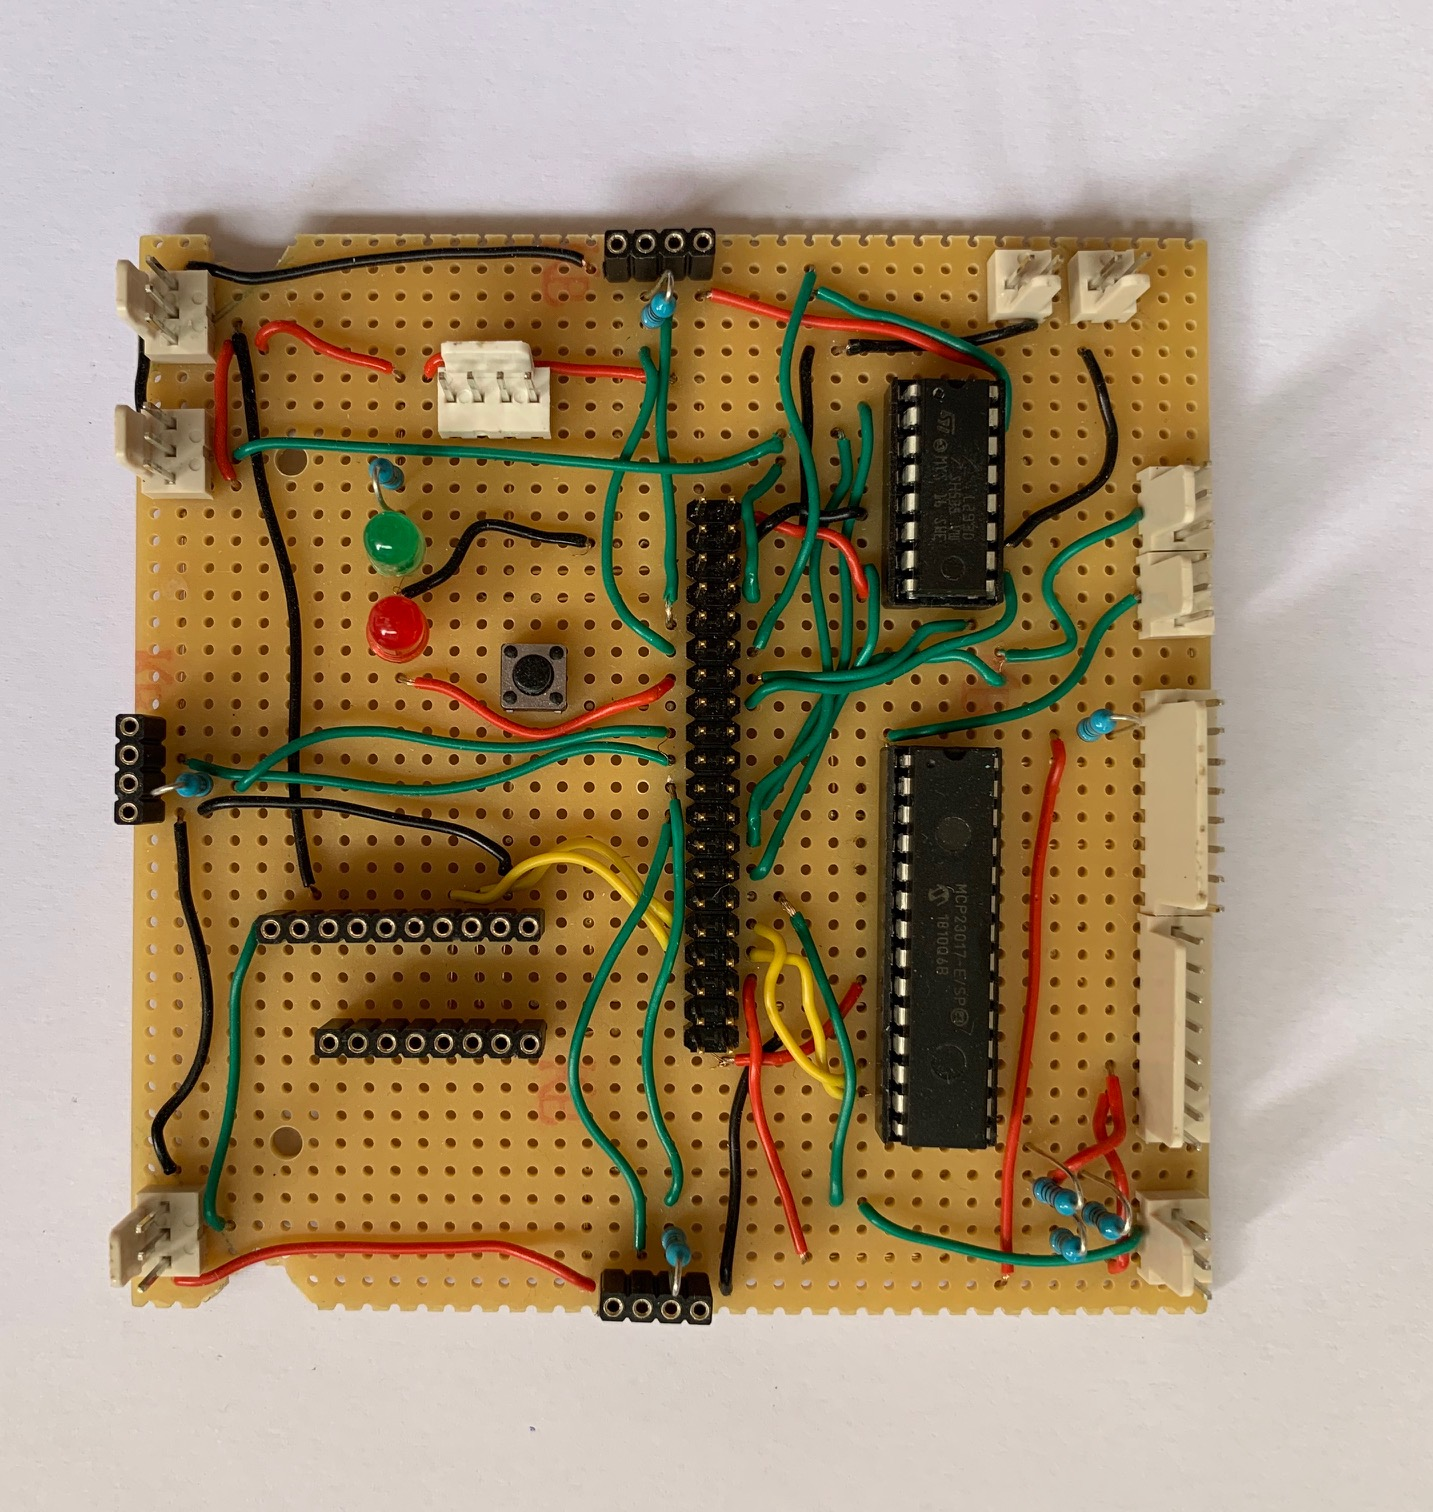
\includegraphics[width=5cm]{images/sensorplatte_unbestueckt.jpg} }}%
		\qquad
		\subfloat[Sicht auf die Lötstellen]{{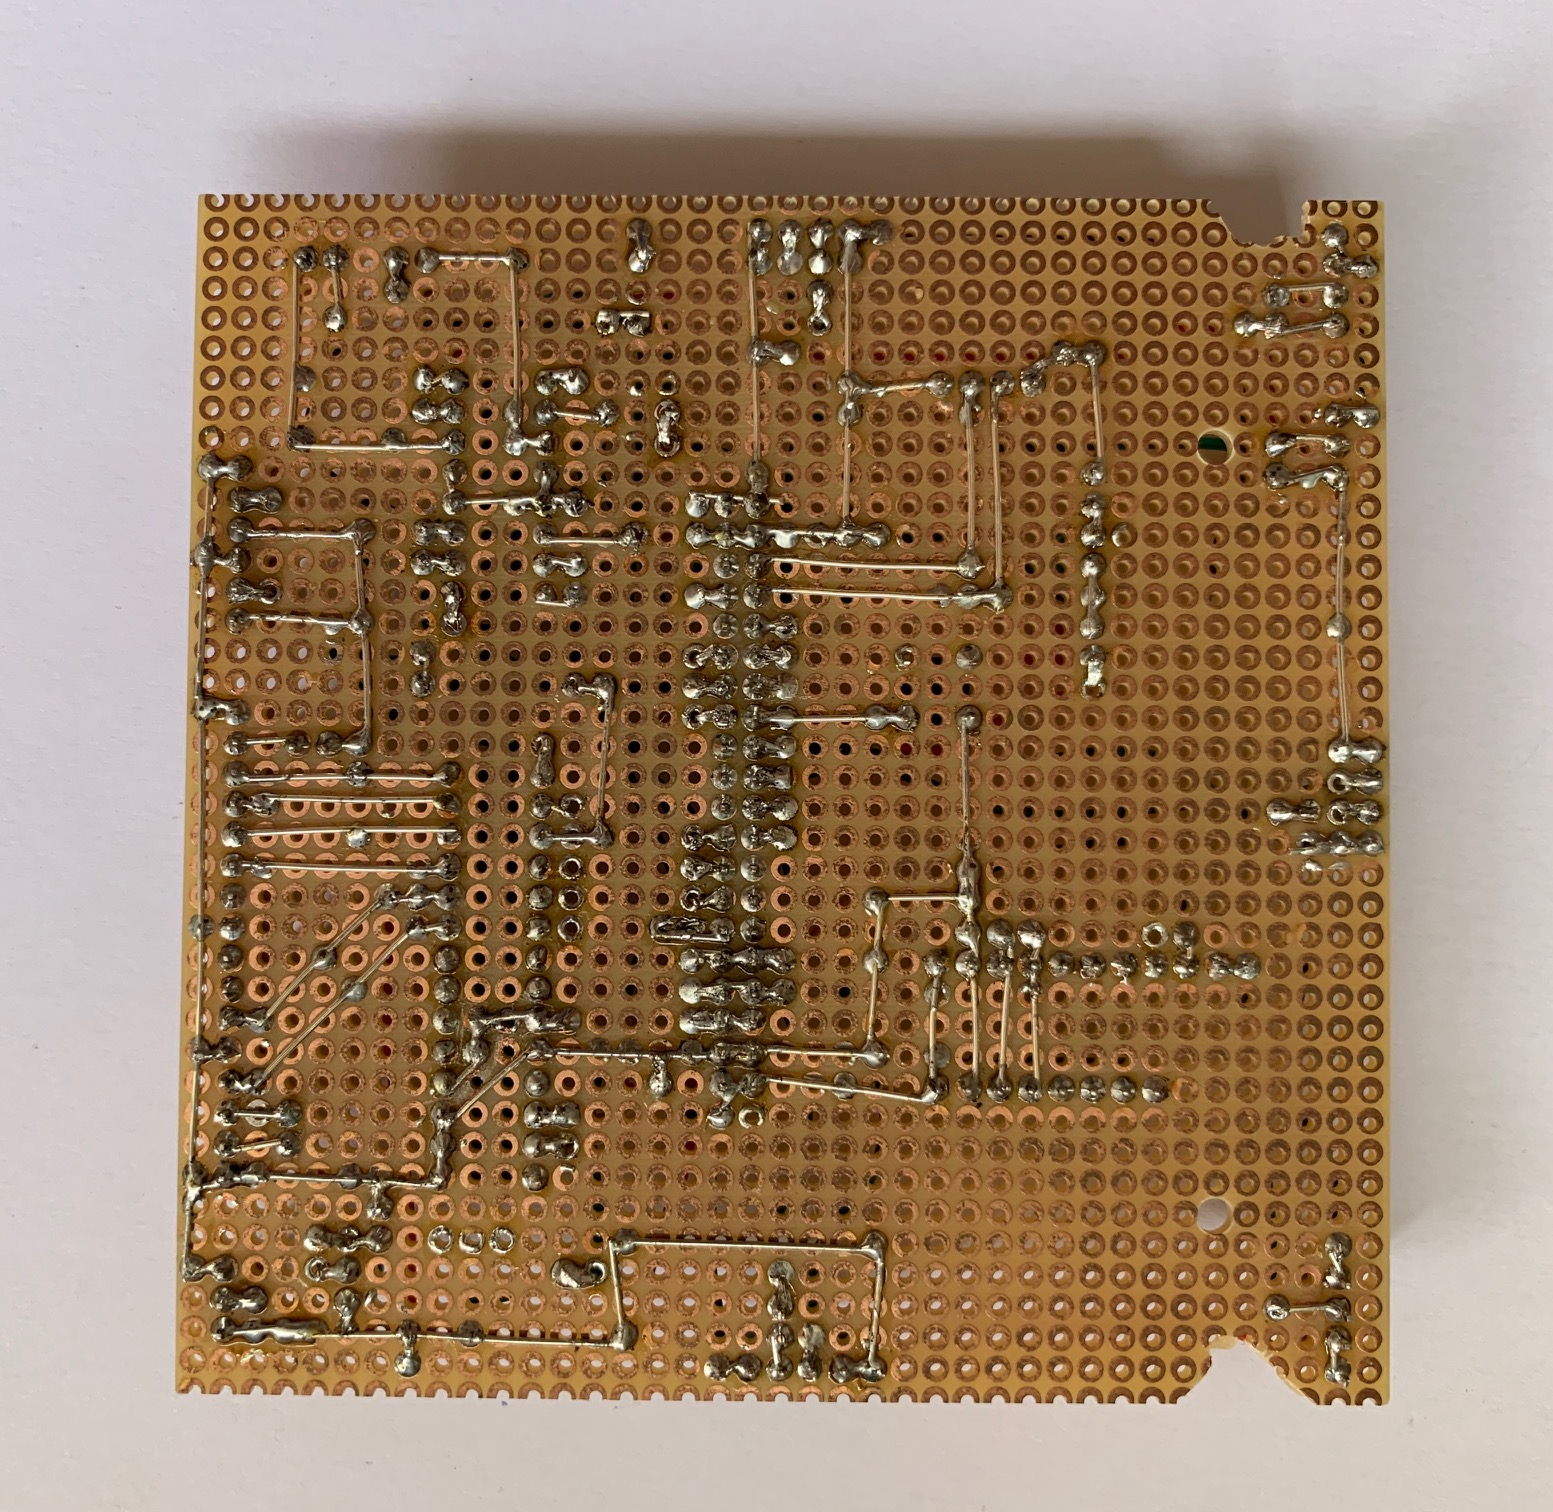
\includegraphics[width=5cm]{images/sensorplatte_hinten.jpg} }}%
		\qquad
		\subfloat[Bestückte Sensorplatte]{{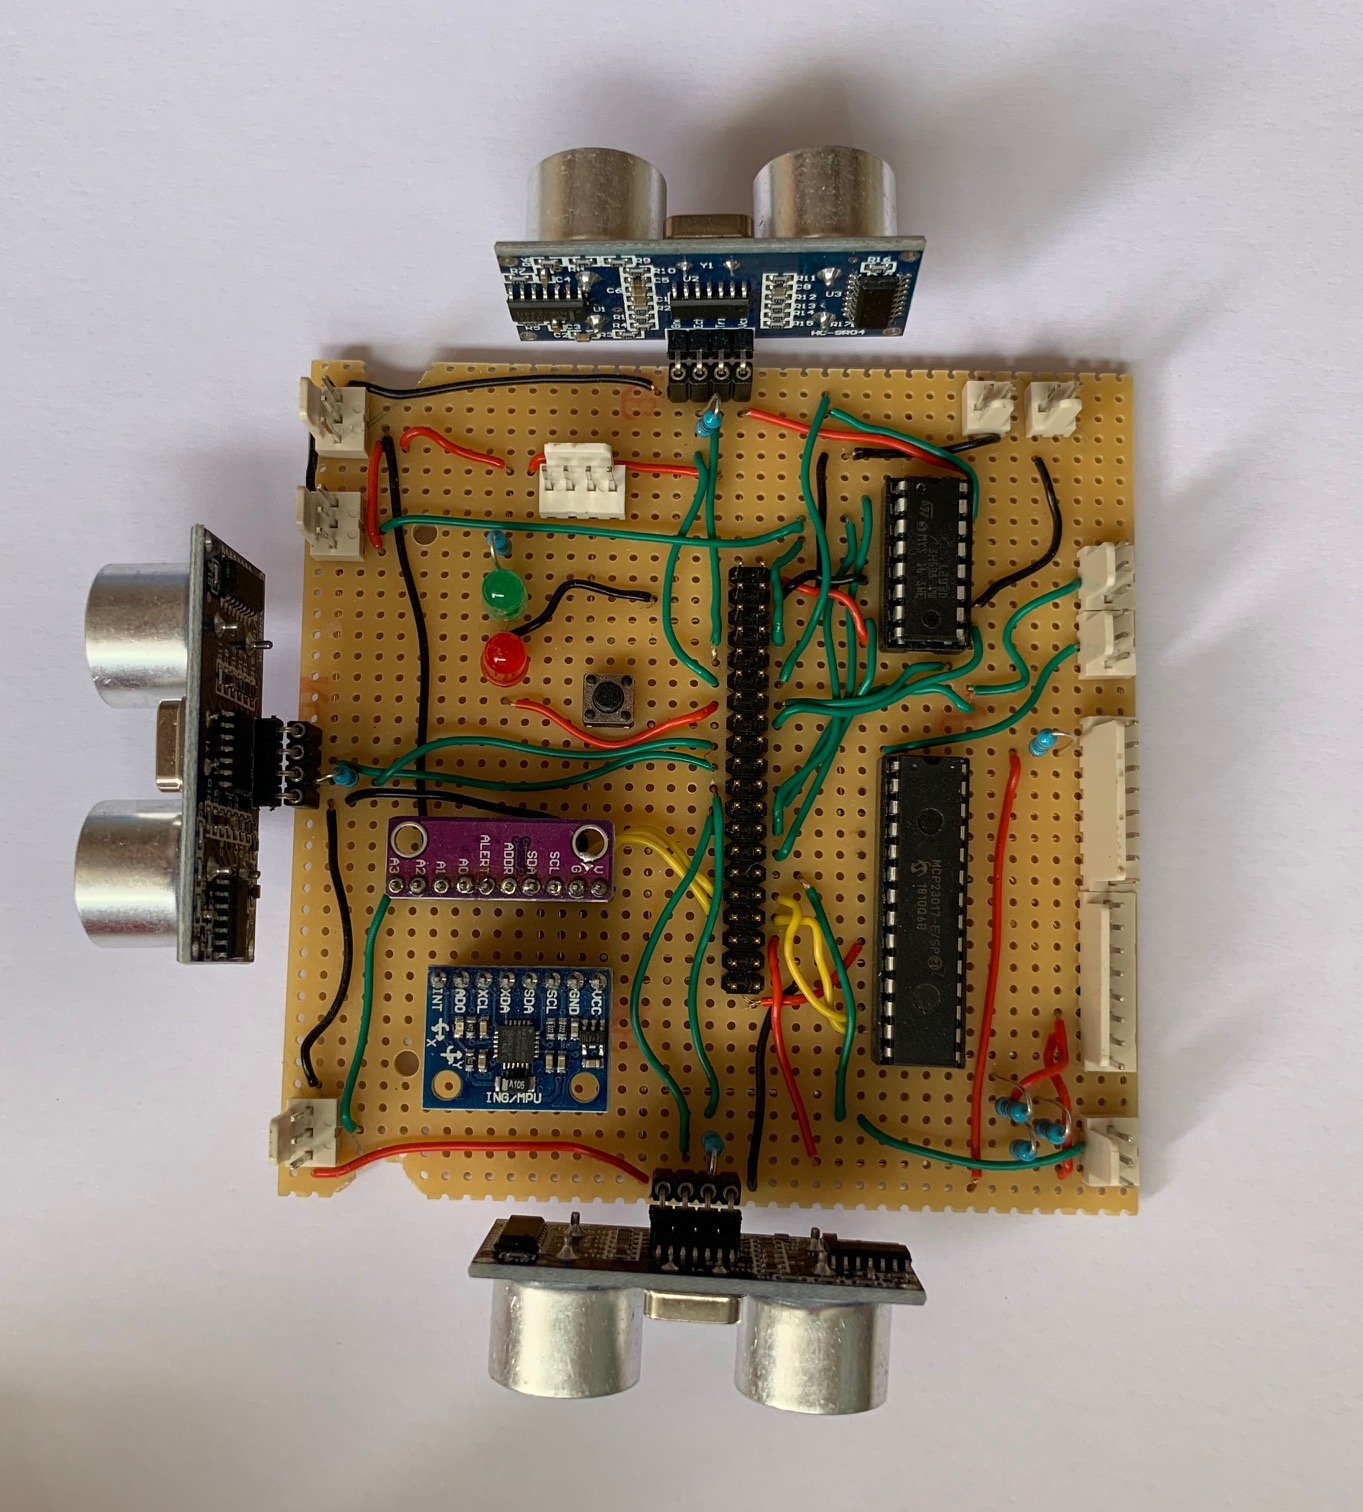
\includegraphics[width=5cm]{images/sensorplatte_bestueckt.jpg} }}%
		\qquad
		\subfloat[Verkabelte Sensorplatte]{{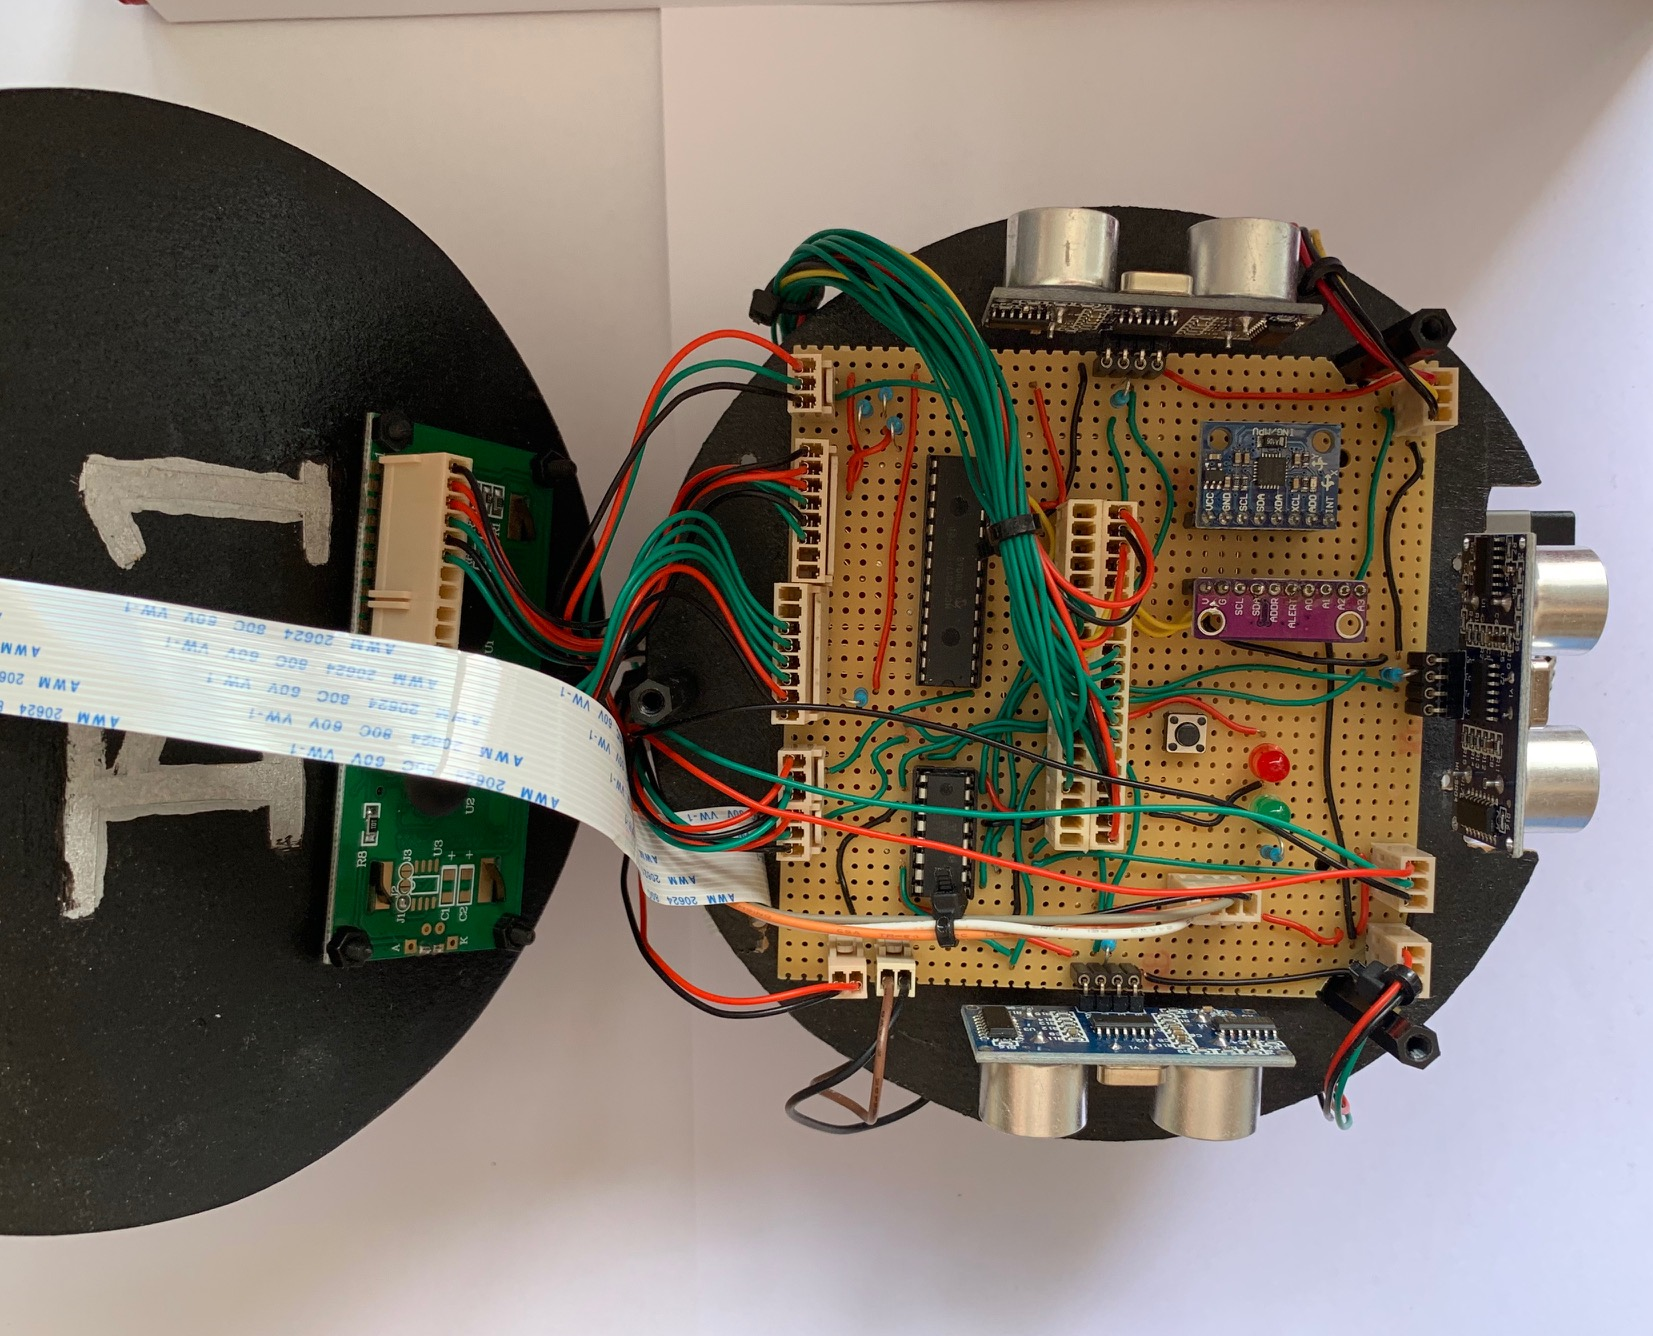
\includegraphics[width=5cm]{images/sensorplatte_verkabelt.jpg} }}%
		\caption{Die fertige Sensorplatte}%
		\label{fig:Sensorplatte}%
	\end{figure}
	
	\FloatBarrier
	% ganze Kapitel 10 Seiten max
	\section{Software-Framework}
	Ein Software-Framework sollte die einfache Bereitstellung von Funktionen bieten. Das Roboter-Framework sollte so ermöglichen, dass ein Anwender die Treiber für die Sensorik nicht selbst schreiben muss, sondern sich die benötigten Daten vom Framework bereitstellen lässt. Dies erlaubt ein schnelleres Entwickeln von Anwendungen für den Roboter ohne ein explizites Management der Hardware-Funktionalität. 
	
	\begin{figure}[!htb]
		\centering
		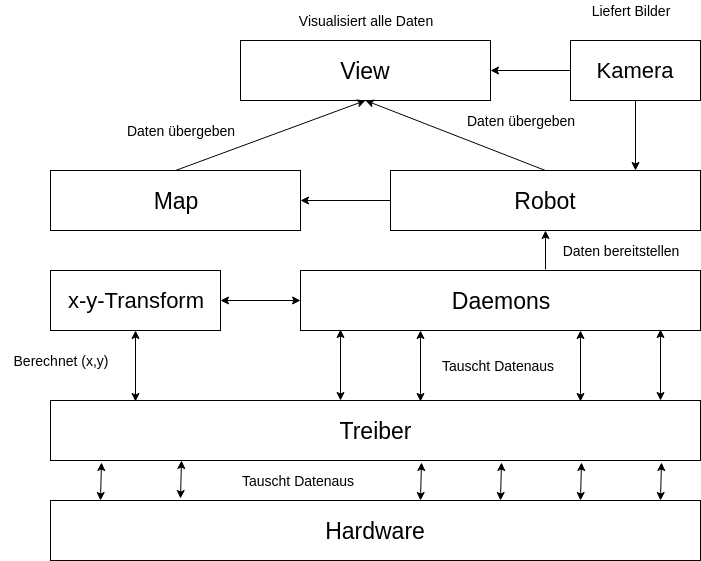
\includegraphics[scale=0.50]{images/Framework.png}
		\caption{komplettes Framework}
	\end{figure}
	
	\subsection{Python}
	Das entwickelte Framework nutzt als Sprache Python. Python ist ursprünglich als reine objekt-orientierte Skriptsprache zum Ausführen kleiner Aufgaben und Funktionen entwickelt worden. Mit Python 2 wurde die Funktionalität der Sprache so erweitert, dass sie nun die gleichen Projekte realisieren kann, die auch andere Hochsprachen verwirklichen. \\
	Python erlaubt kleine Skript-Dateien miteinander zu kombinieren und ermöglicht damit größere Programme 'zusammen zu bauen'. Diese Modularität erklärt die Popularität von Python. Weiterhin lässt sich Python-Code auf allen Betriebssystemen direkt ausführen und muss nicht maschinen-bezogen programmiert werden. \\
	Python gilt auch als natürliche Sprache der Pi. Diese erlaubt die gesamte Steuerung des Rechners über Python-Skripte. Daher gibt es innerhalb der Pi-Community im Internet eine große Datenbank fertiger Skripte, welche die Programmierzeit erheblich verkürzten, da nicht  jede Funktionalität selbst programmiert werden muss. \\
	In diesem Projekt wird Python 2.7 verwendet, weil dies hoch skalierbar auf Python 3.x ist. Der Weg von 3 auf 2.7 jedoch nicht möglich ist. Damit wird die Funktionalität des Frameworks auch für ältere Pi Modelle gewahrt.
	
	
	\subsection{PyBot- Framework}
	
	\begin{figure}[!htb]
		\centering
		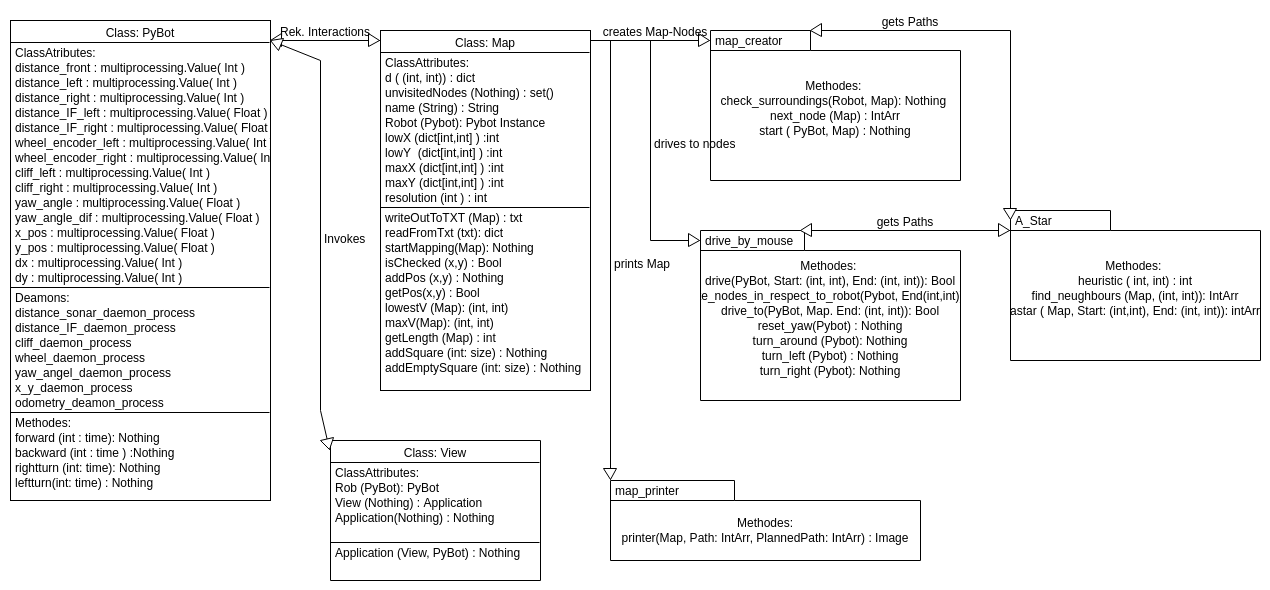
\includegraphics[scale=0.50, angle=90]{images/software.png}
		\caption{Framework als UML-Diagramm ohne Sensorik-Daemons}
	\end{figure}
	
	Das PyBot-Framework wurde speziell für diesen Roboter entwickelt, lässt sich jedoch auf ähnliche Roboter umschreiben. \footnote{näheres im Anhang unter Installation}
	Es ist eine Sammlung von Skripten, welche die Steuerung alle nötigen Sensorik übernimmt und als Funktionen und Klassen dem Nutzer zur Verfügung stellt. Den Kern bildet die PyBot-Klasse. Über diese ist ein einfacher Zugriff auf die Sensorik genauso möglich wie die Steuerung der Motoren. Daneben erlaubt die View-Klasse ein interaktives Steuern des Roboters über ein einfaches grafisches Nutzer-Interface (GUI). 
	\FloatBarrier
	\subsection{Hardware Treiber}
	Die Treiber für die Sensorik wurden entweder komplett selbst geschrieben oder - falls vorhanden - vom Hersteller bezogen und angepasst \footnote{Der Analog-Digital-Wandler verfügt über ein Python-Treiber von Adafruit}. Hierbei lag der Fokus der Software-Entwicklung in einer ausfallsicheren und genauen Verwertbarkeit der Daten. Dazu wurden für alle Abfragen Time-Outs festgelegt, welche endlos-Schleifen verhindern und bei Bedarf die Abfragefolge komplett neu starten. Weiterhin sind Korrektheitstest implementiert, welche unmögliche Werte oder Fehlmessungen direkt im Treiber abfangen. Dies erleichtert das Entwerfen von späteren Applikationen, da derartige Werte nicht zurückgeliefert werden. \\
	Die Ausfallsicherheit ist dabei wichtig, weil die Treiber als Daemons im Roboter agieren. Daemons sind Hintergrund-Aktivitäten des Betriebssystems und der Hardware, welche für den Nutzer nicht erkennbar sind. Sie stellen grundlegende Funktionalitäten bereit und müssen stabil gegen mögliche Fehler innerhalb der Hardware sein. Eine fehlerhafte Meldung oder Dateneintrag eines Daemon ist nicht direkt ersichtlich und führt meist zu unerwarteten Abstürzen oder unerkannten Fehlern. \\
	Die Implementierung als Daemon bietet den Vorteil, dass sich der Nutzer keine weiteren Gedanken über die einzelnen Treiber machen muss. Stattdessen werden Sie ihm als 'System-Werte' zur Verfügung gestellt und der er kann sich auf ihre Korrektheit verlassen. 
	
	
	\subsection{Mapping}
	Die Karte verwaltet das PyBot-Framework über die Klasse Map. Diese teilt sich in eine Hauptklasse und vier Skripte.\\
	Die Karte ist als Grid-Map konzipiert, d.h. eine vollständige Karte besteht aus n Zellen, welche als Tuple aus $(x,y)$-Werten angesprochen werden. Diese repräsentieren Koordinaten im euklidschen Raum. Jede Zelle besteht aus einem einzelnen Belegt-Wert, welcher entweder 0 - frei - oder 1 - belegt - sein kann. Anhand dieser Informationen kann der Roboter seine Umwelt als Karte abbilden und sich in ihr zurecht finden. \\
	Die Klasse Map fungiert hierbei als Interface für alle Funktionalitäten bezüglich dieser Karte. Über sie werden alle Prozesse, wie z.B. das Einfügen einer neuen Zelle, die Ausgabe der Karten-Datenbank als Bild oder das Erstellen einer neuen Karte geregelt. Sie ist dabei in der Lage die Karte zu skalieren und das an alle folgenden Skripte weiterzureichen. Die Skalierung wird zentral aus der Roboter-Klasse übernommen und beträgt im Default 1cm \footnote{D.h. eine Zelle hat die Maße $1cm \times 1cm$}.\\
	Die Karte selbst wird über das Skript $map\_creator $ erstellt. Diese bekommt von der Map Klasse die Informationen über die Karte selbst und von der PyBot-Klasse alle Informationen vom Roboter. Auf Basis dieser Daten baut Sie iterativ eine Karte der Roboter Umgebung auf. Dabei verwendet Sie eine an \cite{Hofmeister} angelegte Strategie: 
	
	\subsubsection{Erstellen der Karte}
	
	\begin{figure}[!htb]
		\centering
		\subfloat[Eine Iteration mit Takt 0.005]{{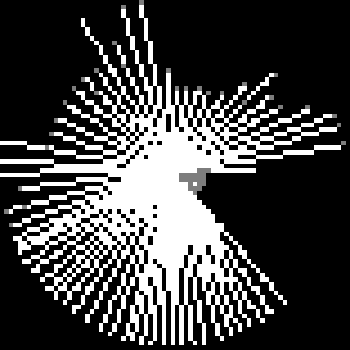
\includegraphics[width=5cm]{images/map1.png} }}%
		\qquad
		\subfloat[Eine Iteration mit Resolution 5cm]{{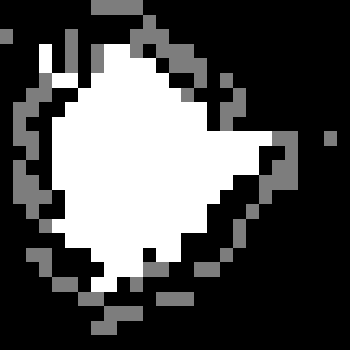
\includegraphics[width=5cm]{images/map2.png} }}%
		%\qquad
		%\subfloat[Bestückte Sensorplatte]{{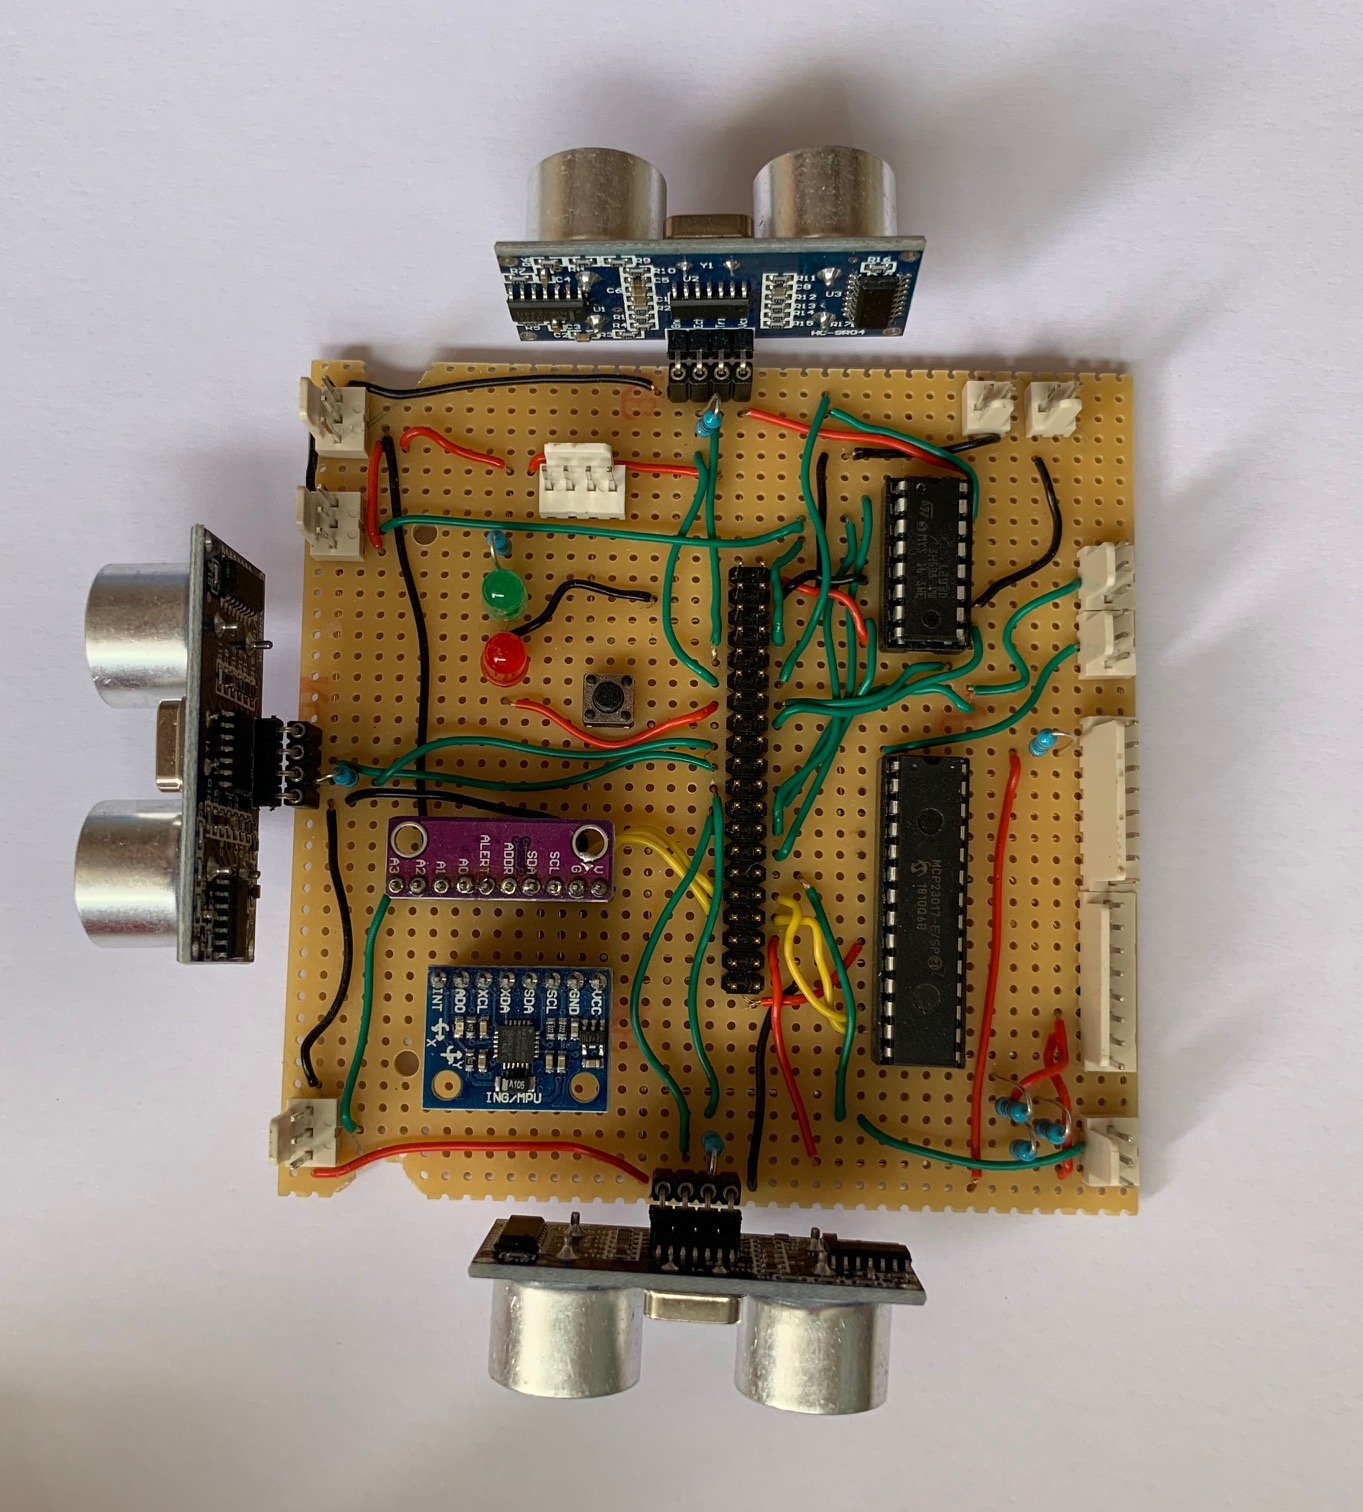
\includegraphics[width=5cm]{images/sensorplatte_bestueckt.jpg} }}%
		%\qquad
		%\subfloat[Verkabelte Sensorplatte]{{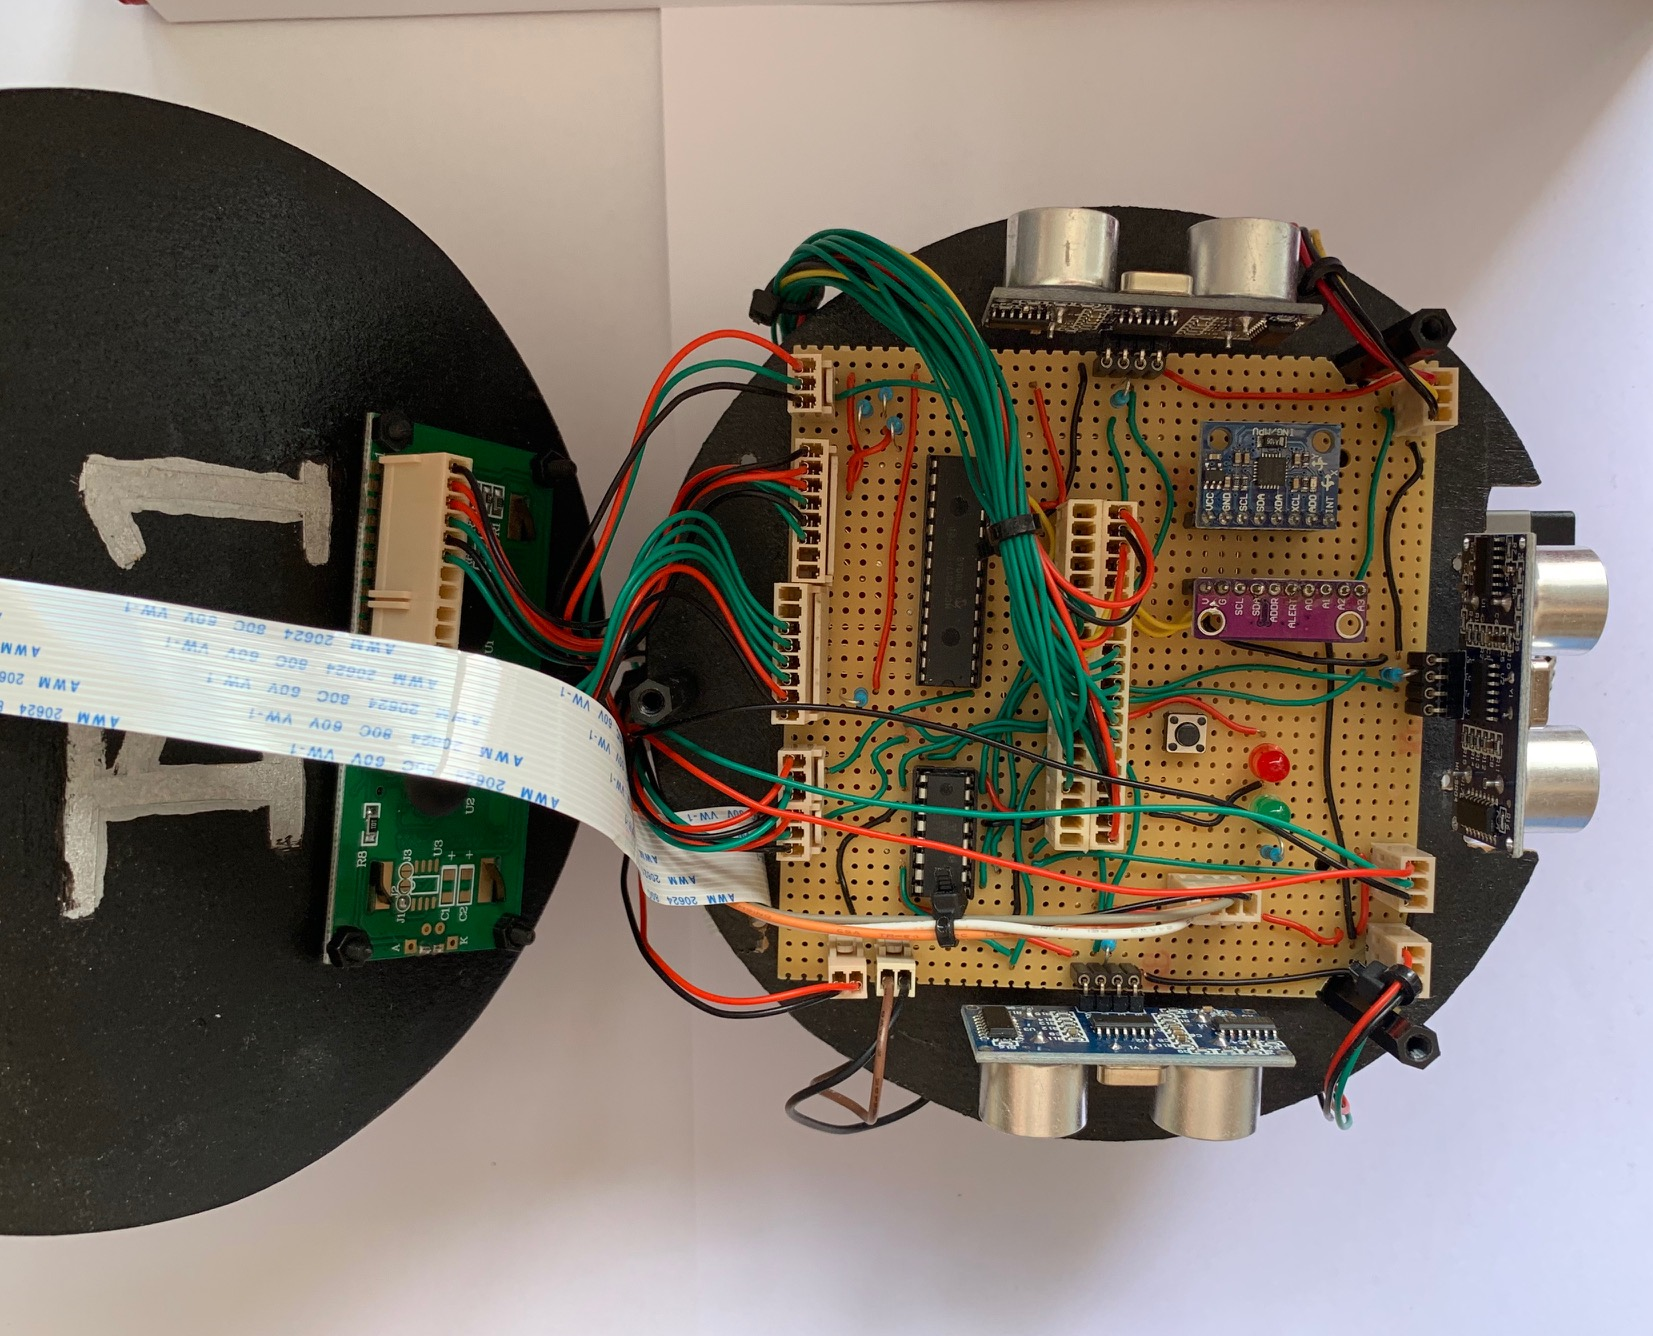
\includegraphics[width=5cm]{images/sensorplatte_verkabelt.jpg} }}%
		\caption{verschiedene Karten}%
		\label{fig:Karten}%
	\end{figure}
	
	Wird der Roboter angeschaltet, so speichert er seine Position als absoluten Referenzpunkt mit den x,y-Werten $(0,0)$. Der erste Punkt bildet im folgenden Mapping den Ursprung, von welchem sich die Karte aufbaut. \\
	In der ersten Iteration dreht sich der Roboter einmal vollständig um die eigene Hauptachse. Dabei misst er im Takt von 0.0005s den Abstand mit Hilfe der beiden vorderen IF-Sensoren. Diese Daten interpretiert der Algorithmus nun als Vektor von seiner jetzigen Position mit Länge m und einem Yaw-Winkel $\psi$. Falls der Vektor eine Länge größer 40cm hat, so wird definiert, dass er auf keinen Gegenstand gestoßen ist. Beträgt die Länger weniger als 40cm, so ist bei $m_i$ ein Gegestand und die jeweilige Zelle besetzt. Da die IF-Sensoren eine Minimaldistanz von 10cm haben, wird jeder Strahl mit einer Messung des Ultraschallsensors begleitet. Dieser kann auf 4cm exakt messen und sollte ein Gegenstand noch näher sein, so liefert der Sensor Fehlermeldungen. \\
	Der einzelne Vektor wird - mit Hilfe des Satzes von Pythagoras - in Zellwerte $\vec{(x,y)}$ umgerechnet:
	
	\begin{align}
	x_\text{end} &= x_\text{Robot Position} + m * sin(\psi)\\
	y_\text{end} &= y_\text{Robot Position} + m * cos(\psi)
	\end{align}
	Jede Zelle welche der Vektor passiert hat, wird in die Kartendatenbank aufgenommen mit dem Wert 0 (frei) und die Zelle am Ende des Vektors als 0(frei), falls der Vektor länger als 40cm war oder als 1 (besetzt), falls der Vektor kürzer war als 40cm aber länger als 4cm. Beträgt die Länge des Vektors weniger als 4cm, so ist - theoretisch - keine Aussage möglich, wird in diesem Algorithmus der Wert auf 1 gesetzt. \\
	Nachdem der Roboter eine Umdrehung getätigt hat, verfügt er über eine kreisrunde Karte seiner Umgebung mit dem Radius 40cm. \\
	Alle freien Zellen werden in einem Python-Set verwaltet. Nach jeder Kreis-Iteration wird das Set gefiltert, so dass keine freien Zellen mehr enthalten sind, welche durch ihre Nachbarn abgedeckt sind oder deren Nachbarn 'Wände' und bereits erkundete Zellen sind. Ziel davon ist es, dass nur die freien Zellen am Rand des Kreises enthalten bleiben, welche nicht durch Gegenstände blockiert werden. Ist das Set nach einer Iteration leer, so weiß der Roboter, dass die Karte fertig erstellt wurde. \\
	Befinden sich im Set noch Knoten, so berechnet der $map\_creator$ mit einer Heuristik die nächste zu erkundende Zelle. Die Heuristik wählt dabei die Zellen am Rande der x-Achse des zuletzt ausgeführten Kreises, falls dieser mindestens 30cm entfernt liegt. Sollte dies nicht so sein, sucht sie eine Zelle aus dem letzten Kreis, welche diesen Mindestabstand hat. Wird keine gefunden, so wird der nächste freie Punkt mit höchster Manhattan-Distanz gewählt. Durch diese Heuristik soll eine möglichst schnelle und weite Abdeckung des Raumes erfolgen. \\
	Die Überdeckung einer freien Fläche kann zeit- und bewegungs intensiv werden, wie das Bild veranschaulicht. Daher sollte die Heueristik vermeiden, dass zu viele Wege gefahren werden. Die exakte Abdeckung einer Fläche mit Kreisflächen lässt sich genauer durch Algorithmen bestimmen \footnote{wobei hier darauf zu achten ist, dass nicht jede Lösung implementierbar ist. Pack- und Füllprobleme lassen sich meist auf NP-vollständige Probleme reduzieren, womit eine exakte Lösung - in der Realität -  nicht möglich ist. }, diese sind für diesen Zweck jedoch zu rechenintensiv und haben Voraussetzungen, welche nicht erfüllt werden können. So ist die genaue Raumgröße zu Beginn unbekannt. Ebenso die Raumaufteilung. Eine Heueristik wie hier muss daher eine grobe Abschätzung bleiben. 
	\begin{figure}[!htb]
		\centering
		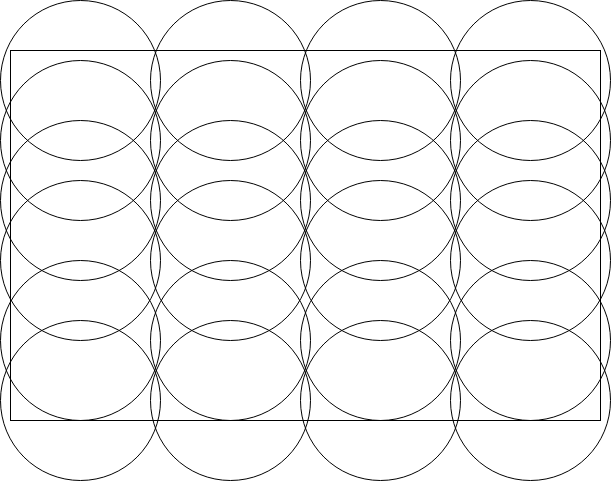
\includegraphics[scale=0.25]{images/Kreis.png}
		\caption{Kreisabdeckung}
	\end{figure}
	
	\FloatBarrier
	\subsubsection{weitere Map Skripte}
	Die Map-Klasse kann auf einen klassischen A*-Algorithmus zurückgreifen. Dieser operiert schnell auf den verwendeten Python-Dictionarys und Sets. Dabei werden exakte Routen über freie Zellen von einem Start zu einem Endknoten geliefert. \\
	Das Printer Skript visualisiert die Karten-Datenbank für den Menschen. Sie ist dabei in der Lage die Position des Roboters, geplante  und beschrittene Pfade mit einzuzeichnen.\\
	Während $Drive\_by\_Mouse$ ein Skript ist, welches die Motorsteuerung innerhalb der Map Struktur übernimmt. Dabei wird auf die PyBot-Klasse zurückgriffen, nur dass mit genauen Motorsignalen die Fahrbefehle auf Basis der Daten der Roboter-Odometrie erfolgen. Dadurch ist es innerhalb der Map Skripte möglich, dass Befehle wie 'Go to Position (x,y)' realisiert werden können. 
	
	% ganze Kapitel 10 Seiten max
	\chapter{Evaluierung}
	\section{Hardware}
	\subsection{Roboter Aufbau}
	Der Aufbau des Roboters wurde vom Ct'Bot übernommen. Dies zeigte bereits bei diesem bekannte Nachteile. So ist es dem Roboter nicht möglich Gegenstände die hinter ihm liegen zu erfassen oder Hindernisse zu erkennen, welche seitlich auf ihn zu kommen. Dies muss über die Steuerung geregelt werden. Daher ist ein Rückwärtsfahren ohne vorherige Drehung zum Scannen der Fläche hinter dem Roboter nicht möglich. \\
	Ein weiteres Problem liegt in der geringen Bodenfreiheit der Bodenplatte. Diese lagert auf den beiden Rädern, sowie einer Kunststoffkugel vorne und hinten. Durch diese Kugeln kann es passieren, dass der Roboter in Teppichen 'gefangen' wird und nicht mehr aus eigener Kraft fahren kann. Weiterhin ist der Maus-Sensor etwas tiefer als die Bodenplatte angebracht. Dies ist nötig um genaue Messwerte zu erhalten. Deshalb beträgt die Distanz zum Boden in der Mitte des Roboters nur 0.2cm. Besonders bei Unebenheiten im Untergrund hebt die Lippe des Maus-Sensors die Räder vom Boden ab und verhindert so weitere Bewegungen. \\
	Der Einsatzbereich des Roboters schränkt sich hierdurch auf glatte Flächen ein. 
	
	\subsection{Distanzsensoren}
	Die beiden Sharp Distanzsensoren wurden zu Beginn geeicht. Dies geschieht durch Distanzmessung  mit dem Sensor bei bekannter Distanz und notieren der Ausgangsspannungen am Sensor. Dies muss für Distanzen ab 10 cm und dann jeweils um 5cm steigent getan werden. Danach wird eine Funktion an die Werte angepasst. Diese Funktion bekommt danach die analogen Output-Werte und ermittelt die Distanze in Zentimetern. Es zeigte sich, dass der Sensor große Ungenauigkeiten liefert, wenn sich die Umwelt ändert. Die Werte änderten sich bei Veränderung der Temperatur und bei Umgebungslichtwechsel. Eine sehr große Rolle spielte die Fläche, besonders das Material und die Farbe, auf die der IF-Strahl traf. Dies bewirkte Fehlmessungen von bis zu 10cm. Kaum zu kontrollieren waren Farbwechsel auf kleinsten Flächen. Im Datasheet von Sharp wird dies explizit erwähnt und jede Messung hier ausgeschlossen:\footnote{Aus dem Datasheet des Sensors} 
	\begin{figure}[!htb]
		\centering
		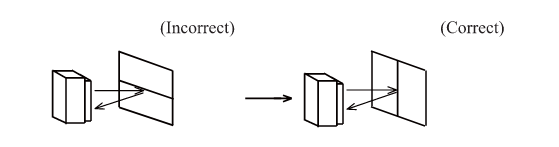
\includegraphics[scale=0.5]{images/sharp2.png}
		\caption{Sharp Anleitung zu unterschiedlichen Materialien}
	\end{figure}
	
	Diese Einschränkung wurde durch die Software teilweise eingefangen, indem Messwerte mit zu großen Distanzsprüngen ignoriert wurden und eine erneute Messung vorgenommen wurde. Sollte diese den gleichen Wert wie zuvor liefern, so galt das als vertrauenswürdig. Dies verhindert zumindest einen Teil der schlimmsten Messfehler. \\
	Weiterhin erreichte keiner der beiden Sensoren die angegebene Messweite von 120cm. Beim linken Sensor lag die max. Reichweite bei 95cm, beim rechten Sensor bei 112cm. Es zeigte sich jedoch, dass die angepasste Funktion bei Werten über 60cm Schwankungen von bis zu 5cm in der Genauigkeit entwickelte. \\
	
	Die Ultraschallsensoren hatten keinerlei Probleme mit der Raumform- oder Farbgebung. Sie funktionieren schnell und auf 1cm genau. Der chinesische Hersteller der Ultraschallsensoren gibt eine Maximaldistanz von 400cm an. Diese konnte nicht erreicht werden. Die verwendeten Ultraschallsensoren hörten ab 50cm auf zuverlässige Werte zu liefern. Ebenso wurde die Mindestdistanz von 2cm nicht erreicht und man muss mit 4 cm rechnen. Abgesehen hiervon leiden die Ultraschallsensoren an Interferenzen miteinander. Dies passiert vor allem dann, wenn sie auf engstem Raum zeitgleich getriggert werden. In solchen Fällen wurde keinerlei Distanz ermittelt. Innerhalb der Software wird daher jeder Ultraschallsensor nacheinander angesteuert und niemals zeitgleich. Dies verhindert die meisten - jedoch nicht alle - Interferenzen. 
	
	\subsection{Maus-Sensor}
	Der Maus-Sensor arbeitet auf 0.6mm genau. Dies konnte im Test nicht ganz erreicht werden, jedoch waren korrekte Ergebnisse ab 1cm gegeben. Daher wurde die Auflösung des Roboters und der Karte nie unter diesem Wert gemessen. Der Vorteil des Sensor war, dass sich die Fehler nicht aufsummierten. Jede einzelne Messung war für sich auf die Auflösung exakt. Zu Problemen führte hingegen der begrenzte interne Speicher des Sensors. Dieser speichert die Differenz der x oder y Bewegung seit der letzten Abfrage als doppelter Hexadezimal-Wert. Dadurch hört der Sensor auf zu arbeiten, falls dieser Wert 127 übersteigt oder unter -128 fällt.\footnote{Datasheet ADNS2610 Avago} Ein sehr schnelles Abfragen der Werte ist unumgänglich, da sonst die Positionswerte nicht mehr stimmen. Die Raspberry Pi war dazu nicht in der Lage, falls der Roboter in voller Geschwindigkeit gefahren ist. Daher wird die Geschwindigkeit gedrosselt, sobald ein Abruf der Positionswerte entweder -127 oder 126 beträgt. Dadurch wird ein Speicherüberfluss im Sensor vermieden.  
	
	\subsection{Gyroskop}
	Beim Gyroskop stellte sich heraus, dass eine Schwankung von 0.8 Grad im Ruhezustand auftritt. Lässt man den Roboter in einer Ruheposition stehen und misst den Sensor aus, so fällt und steigt dieser Kontinuierlich im Intervall $[-0.5, 0.8]$. Dem Datenblatt des Herstellers zufolge, liegen diese Schwankungen im Normbereich und müssen über die Software ausgeglichen werden. Dies wurde innerhalb des Daemons so realisiert, dass dieser erst Veränderungen des Yaw-Winkels übernimmt, die eine Schwelle von 0.8 Grad übersteigen. Daher ist die Genauigkeit der Pose beschränkt. Dies fällt zu Beginn kaum auf, jedoch lässt sich bei der Kartierung beobachten, dass die Winkelfehler sich über die Zeit aufsummieren und bei mehr als 20 Iterationen in der Mapping-Funktion zu Fehlern führen, welche die Karte verzerren. \\
	
	\subsection{Diskussion und Bewertung}
	Die Sensorik ist - trotz des Alters oder der Preisklasse - zuverlässig und ermöglicht innerhalb eines 40-50cm Bereichs eine exakte Vermessung der Roboterumwelt. Bei einem Roboter mit 7.5cm Radius ist dies als ausreichend anzusehen und ermöglicht weitreichende Einsätze und Verwendungen. Die Genauigkeiten bei 1-2 Grad lassen jedoch den Yaw-Sensor zu einem Problem werden, falls der Roboter über einen größeren Zeitraum Fehlerwerte aufsammelt. Dies muss mit weiteren Software-Anpassungen berücksichtigt werden. \\
	Eine Verbesserung der Hardware wäre nur mit einem größeren Sprung innerhalb des Preises möglich und würde sich hier nicht rechnen. Die Sensorik erfüllt den erwarteten Zweck mit geringen Einschränkungen in der Steuerung. 
	
	\section{Map}
	\subsection{Testumgebung}
	Die Kartierung wurde in einem $100cm \times 100cm$ großen, rechteckigen Bereich getestet. Dieser Raum sollte möglichst exakt erfasst werden. Dieser Test wurde mit einem leeren Raum und einem Raum mit Hindernissen ausgeführt. 
	
	\subsection{Ergebnis}
	Der Roboter brauchte für die Kartierung x Zeit. Dabei zeigte sich, dass Fehler in der Distanz- und Positionsmessung eine Verzerrung des Raumes verursachten. Jedoch wurde das Hindernis erkannt und beim weiteren Erkunden umfahren. 
	
	\subsection{Diskussion und Bewertung}
	Der primitive Kartierung-Algorithmus ist in der Lage die Roboter Umgebung zu erkennen und als Karte aufzufassen. Die Dauer und Genauigkeit kann es nicht mit modernen SLAM-Algorithmen aufnehmen, jedoch erfüllt sie ihre Aufgabe ausreichend. Ein Problem ist die Dauer der Kartierung. Ist die Fläche kleinteilig aufgebaut, so erkennt die Heueristik nicht ausreichend gute Wege und fährt infolge dessen viele Wege mehrfach ab. Dies kostet nicht nur Zeit, sondern verschlechtert mit jeder Iteration die Werte in der Bestimmung der Roboter Pose. Es zeigte sich weiterhin, dass die neuesten Werte die Werte der vorherigen Iterationen unzulässig veränderten und durch aufsummierte Fehler in der Positionsbestimmung Hauptverantwortlich waren für falsche Zellen. 
	
	\section{Zusammenfassung}
	Die Roboter Hardware ebenso wie das Software-Framework funktionieren mit größeren Toleranzen in der Exaktheit. Besonders die ältere Hardware scheint weiterhin Nutzbar zu sein und erfüllt die an sie gestellten Aufgaben ausreichend. Viele der Hardware-Probleme können durch Schwellenwerte innerhalb der Software vermindert werden und so zu besseren Ergebnissen führen. Bei der Software zeigte sich, dass der primitive Ansatz keine Karte produzieren kann, welche modernen Maßstäben entspricht. Sie genügte dennoch den eingeschränkten Herausforderungen des PyBot, so dass es möglich war Karten zu erstellen und sich in diesen gezielt zu bewegen. 
	
	
	% 5 Seiten max
	\chapter{Zusammenfassung und Ausblick}
	
	\section{Zusammenfassung}
	
	
	\section{Ausblick}
	
	
	
	
	\appendix
	\chapter{Anhang}
	Im Anhang wird der Zusammenbau des Pybots erklärt. Neben einer genauen Teileliste werden Baupläne und Instalationsanleitungen präsentiert. Dies soll den Leser dazu befähigen die Konstruktion vollständig nachbauen zu können. \\
	Die komplette Software des Python-Framework findet sich unter https://github.com/Nitzsch/PyBot. Ebenso wie eine kurze Einführung in die konkrete Nutzung der verschiedenen Module. 
	
	\chapter{Stück- und Preisliste}
	In diesem Kapitel findet sich eine vollständige Teileliste. Ebenso sind die einzelnen Bezugsquellen aufgezählt und der Preis. Dieser bezieht sich auf den Privatpersonenkauf ohne jeden Rabatt. Oft wurden 5er Packungen gekauft, da dies den Preis des einzelnen Teils enorm senkt. \\
	Nicht aufgezählt sind die Kosten für Lötzinn und Werkzeug. 
	
	\section{Vorhandene Bauteile}
	\begin{center}
		\begin{tabular}{|c|c|c|c|}
			\hline
			Bezeichnung			&Funktion				& Preis	in Euro	&Bezugsquelle\\
			\hline
			L293D				&Motor-Driver-Chip		& 0.37			& vorhanden		\\
			GD2P12				&Infrarot Distanz-Sensor& 10 (2 Mal)	& vorhanden\\
			LCD-Display			&Anzeige				& 8				& vorhanden	\\
			Opti-Flow-Sensor	&Mouse-Bewegungssensor	& 20			& vorhanden\\
			Motor				& DC-Motor mit Aufhängung& 15			& vorhanden\\
			Gummistopper		& Unterseite			& (3Mal)		& vorhanden \\
			330Ohm Res.			&						& 0(5Mal)		& \\
			2k Ohm Res.			&						& 0(2Mal)		& \\
			5k Ohm Res.			&						& 0				& \\
			\hline
			gesammt:			&						&63.37&\\
			\hline
		\end{tabular}
	\end{center}
	
	
	\section{zugekaufte Sensorik}
	\begin{center}
		\begin{tabular}{|c|c|c|c|}
			\hline
			Bezeichnung			&Funktion				& Preis	in Euro			&Bezugsquelle\\
			\hline
			MPU6050				&Gyro					& 1.75			& amazon		\\
			ADS1115				&Analog-Digital-Wandler	& 3.50			& amazon		\\
			MCP23017			&I2C-Multiplex			& 0.95			& reichelt		\\
			Ultraschall-		&Distanzsensor			& 1.7 (3Mal)	& amazon		\\
			TCRT5000			&Infrarot-Sensor		& 1.1 (4Mal)	& amazon		\\
			\hline
			gesammt:			&						&15.7			&\\
			\hline			
		\end{tabular}
	\end{center}
	
	\section{Raspberry Pi und Zubehör}
	\begin{center}
		\begin{tabular}{|c|c|c|c|}
			\hline
			Bezeichnung			&Funktion				& Preis	in Euro			&Bezugsquelle\\
			\hline
			Raspberry Pi 		& Version 3B +			& 32.5			& reichelt		\\
			USB-Kabel			& Stromversorgung		& 3.15			& amazon		\\
			SanDisk Speicher	& Micro-SD, 64GB		& 15			& amazon \\
			Powerbank			& 12kmA					& 16			& amazon \\
			Pi-Camera			&Kamera					& 7				& amazon		\\
			Camera Kabel		&Kabel					& 1				& amazon		\\
			\hline
			gesammt:			&						& 74.65				&\\
			\hline
		\end{tabular}
	\end{center}
	
	\section{Sonstiges Material}
	\begin{center}
		\begin{tabular}{|c|c|c|c|}
			\hline
			Bezeichnung			&Funktion				& Preis	in Euro			&Bezugsquelle\\
			\hline
			Button				&						& 0				& 		\\
			LED					&Anzeige				& 0 (2Mal)		&		\\
			Lochrasterplatte	&Sensorboard			& 0.9			& reichelt		\\
			4Pin Leiste			& 						& 0.2 (3 Mal)	& reichelt		\\
			10 Pin Leiste		&						& 0.5			& reichelt		\\
			8 Pin Leiste		&						& 0.4			& reichelt		\\
			24Pin Dop.-Fed.-L.	&						& 0.1			& reichelt		\\
			16Pin Dop.-Fed.-L	&						& 0.1			& reichelt		\\
			40 Pin Header		&						& 0.6			& reichelt		\\
			2Pin PSK-H			&						& 0.1(2Mal)		& reichelt	\\
			2Pin PSK-H (Fem)	&						& 0.1(2Mal)		& reichelt	\\
			3Pin PSK-H			&						& 0.2(3Mal)		& reichelt		\\
			3Pin PSK-H (Fem)	&						& 0.2(3Mal)		& reichelt		\\
			4 Pin PSK-H			&						& 0.2			& reichelt\\
			4 Pin PSK-H	(Fem)	&						& 0.2			& reichelt\\
			20 Pin PSK-H	(Fem)&						& 0.2 (2Mal)	& reichelt\\
			8Pin PSK-H			&						& 0.3(2Mal)		& reichelt\\
			8Pin PSK-H (Fem)	&						& 0.3(2Mal)		& reichelt\\
			Crimp-Kontakte		& 20er Pack				& 0.3 (min 5)	& reichelt\\
			Holzplatte, MDF 4mm	& Radius 7.5cm			& 0.5(3Mal)		& Baumarkt		\\
			M3 Schrauben		& set mit Abstandshalter& 0(40Mal)		& amazon		\\
			M3 Muttern			& set mit Abstandshalter& 0(20Mal)		& amazon		\\
			Kabellitze			& 3 versch. Farben		& 0.76			& reichelt		\\
			Kabelaufhänger		&						& 0.5(3Mal)		& reichelt		\\
			Gummiband			&						& 0				& baumarkt\\
			Abstandshalter 		& Kunststoff, versch. G.& 2				& amazon		\\
			\hline
			gesammt: 			&						&14.06			&\\
			\hline
		\end{tabular}
	\end{center}
	
	\section{Gesammtpreis}
	\begin{center}
		\begin{tabular}{|c|c|}
			\hline
			Bezeichnung				& Preis	in Euro	\\
			\hline
			Sensorik				& 15.7\\
			Raspberry Pi u. Zubehör	& 74.65\\
			sonstige Bauteile:		& 14.06\\
			\hline
			gesammt:				& 104.41\\
			\hline
		\end{tabular}
	\end{center}
	Viele Preise beziehen sich auf die reduzierten Angebote mit 5 Bauteilen statt einem. D.h. der Preis von 104.41 Euro pro Stück wird nur realisiert, wenn 5 oder mehr gebaut werden. Ansonsten erhöht sich der Preis uU. \\
	Muss der Roboter vollständig neu gebaut werden (ohne die Basis des Ct'Bots) so erhöht sich der Preis entsprechend um 63.37 Euro auf 167.78Euro. 
	
	\chapter{Baupläne}
	\section{obere Platte}
	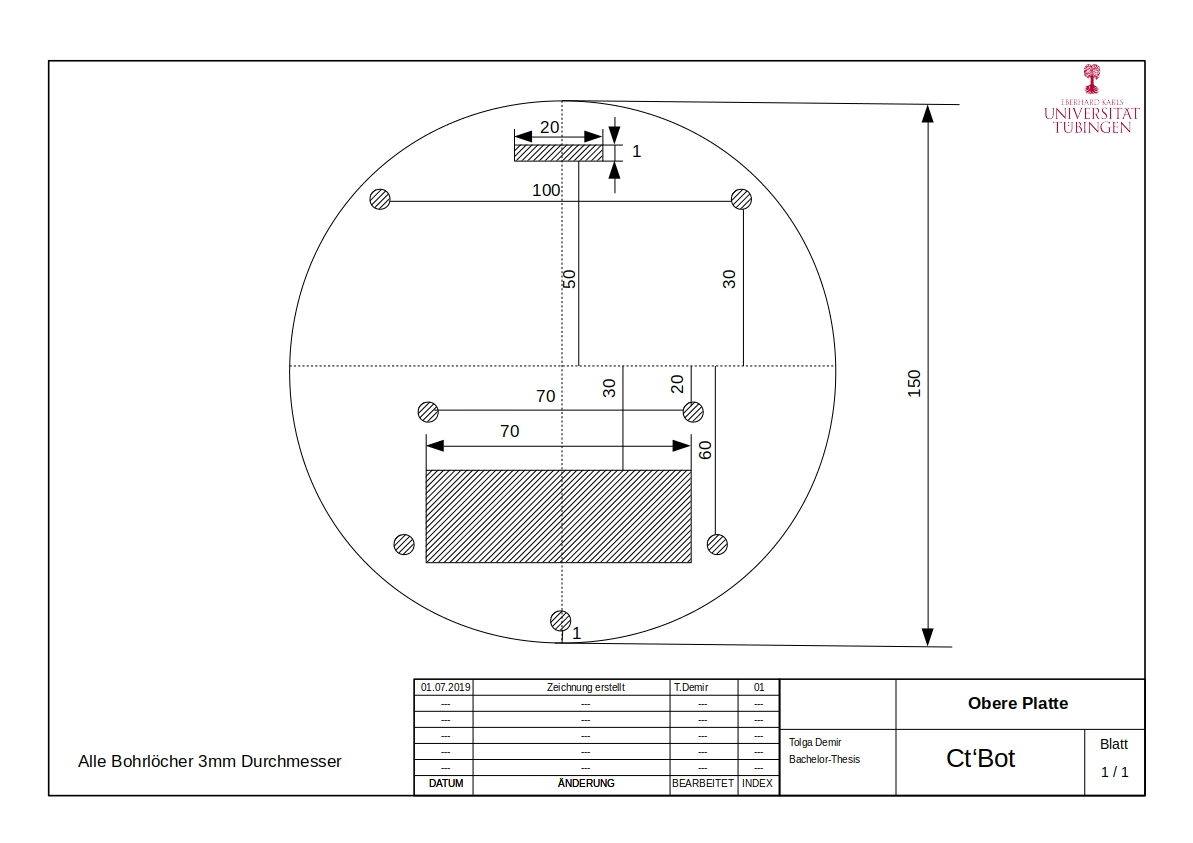
\includegraphics[angle=90,origin=c, scale= 0.5]{images/Zeichnung_obere_Platte.jpg}
	\section{Mittlere Platte}
	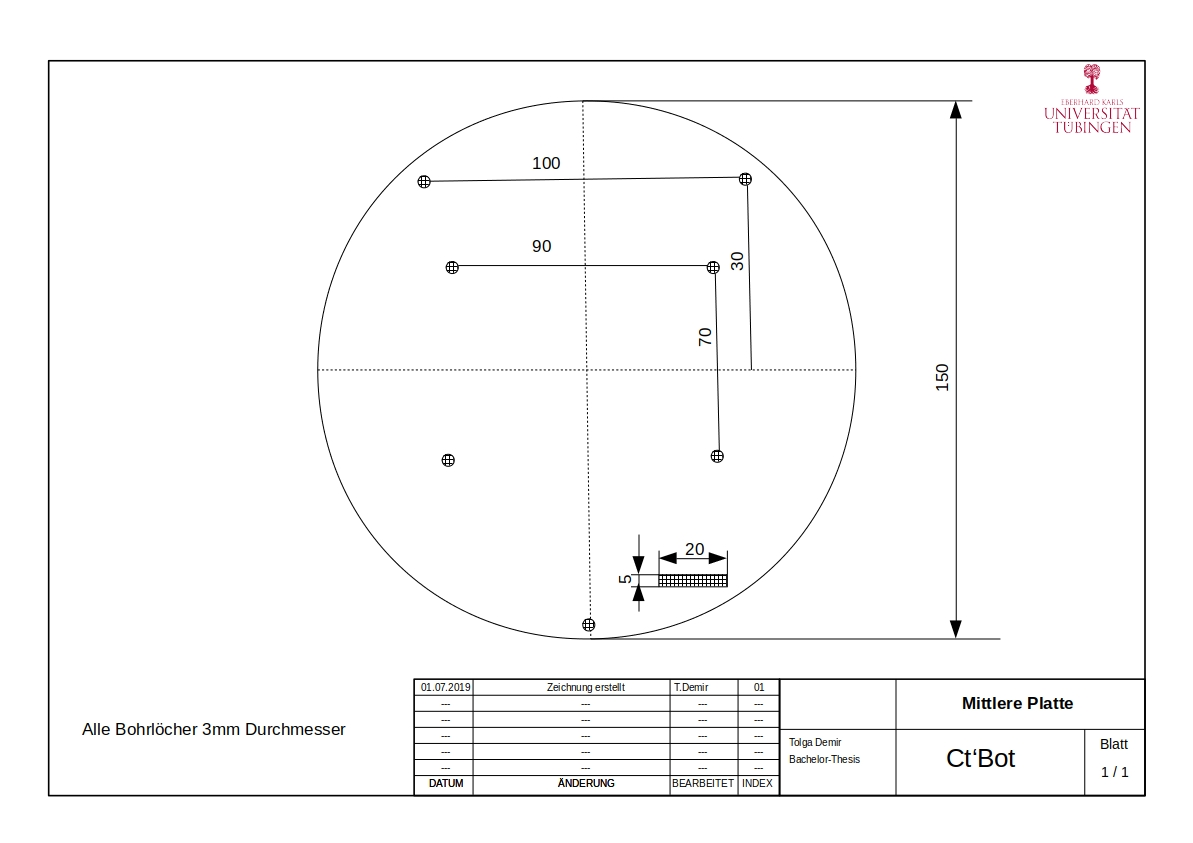
\includegraphics[angle=90,origin=c, scale= 0.7]{images/Zeichnung_mittlere_Platte.jpg}
	\section{Bodenplatte}
	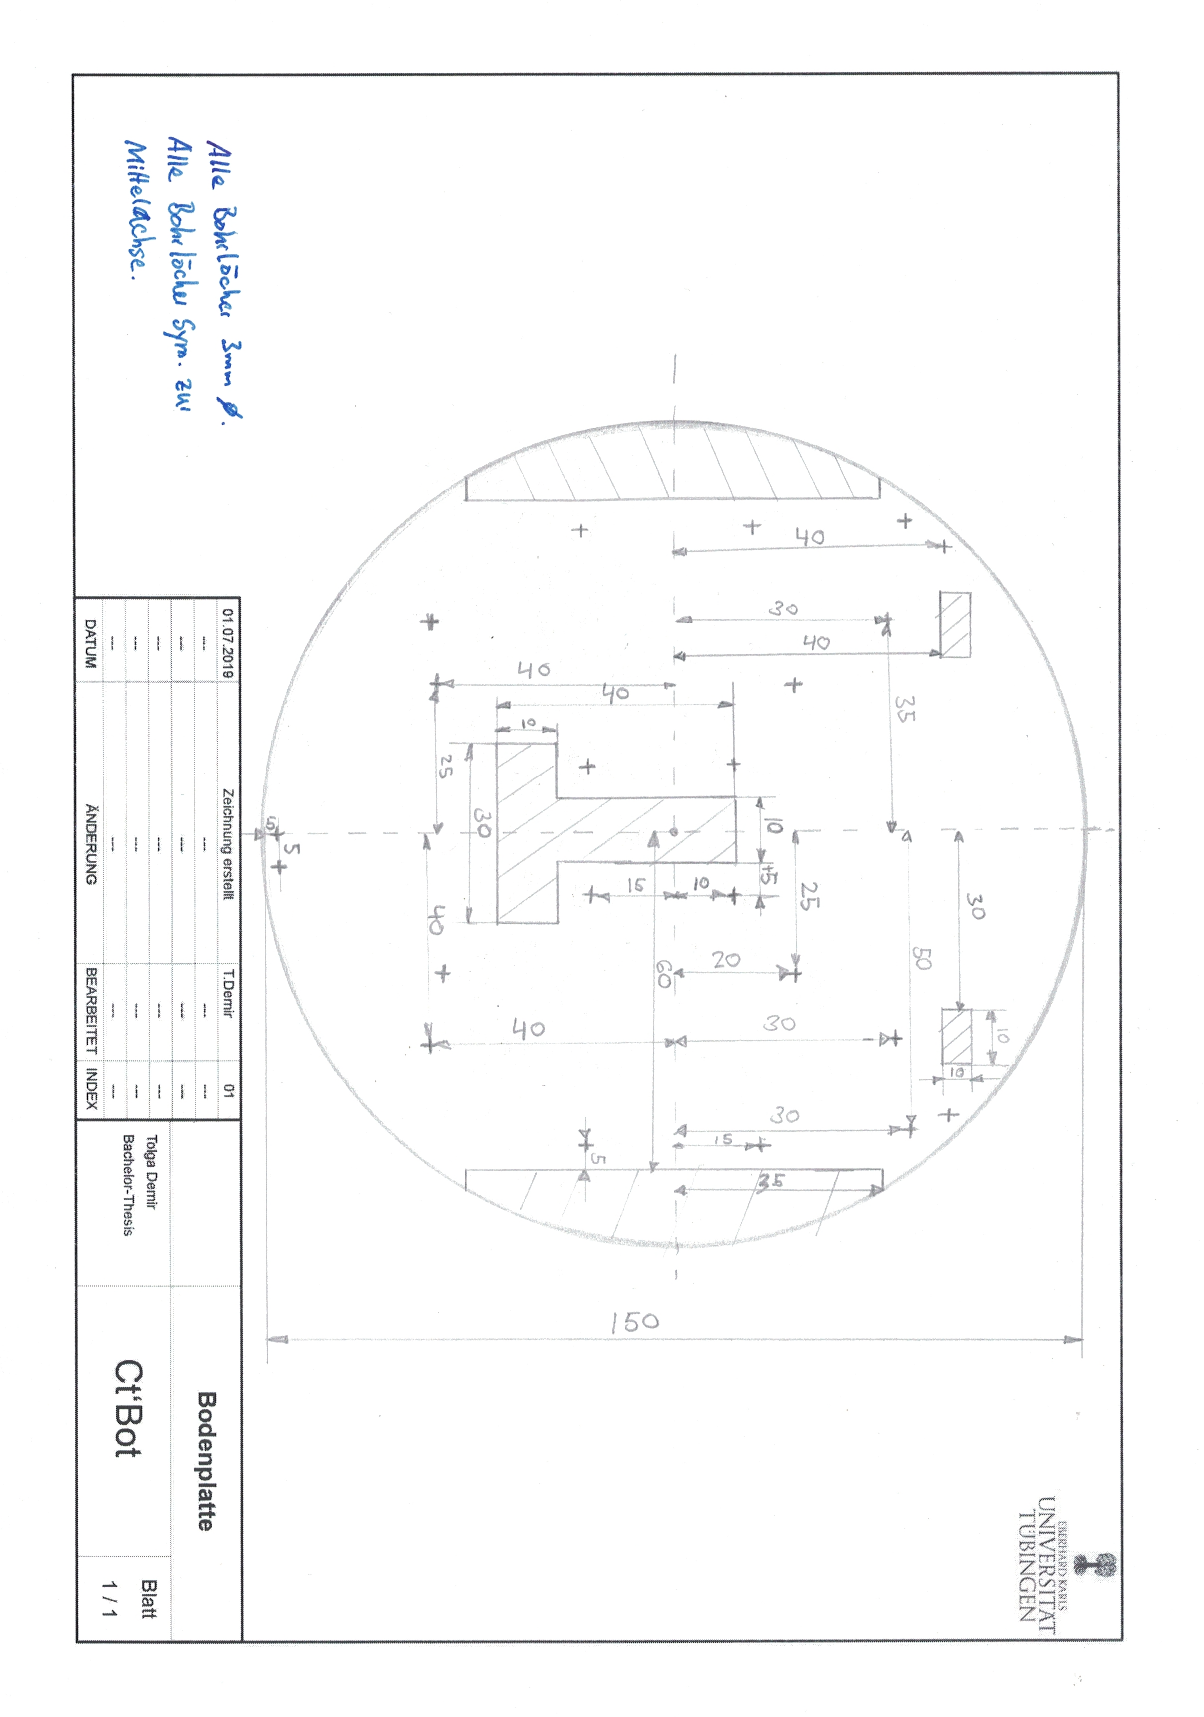
\includegraphics[angle=180,origin=c, scale= 0.7]{images/Bodenplatte.pdf}
	\section{Akku-Träger}
	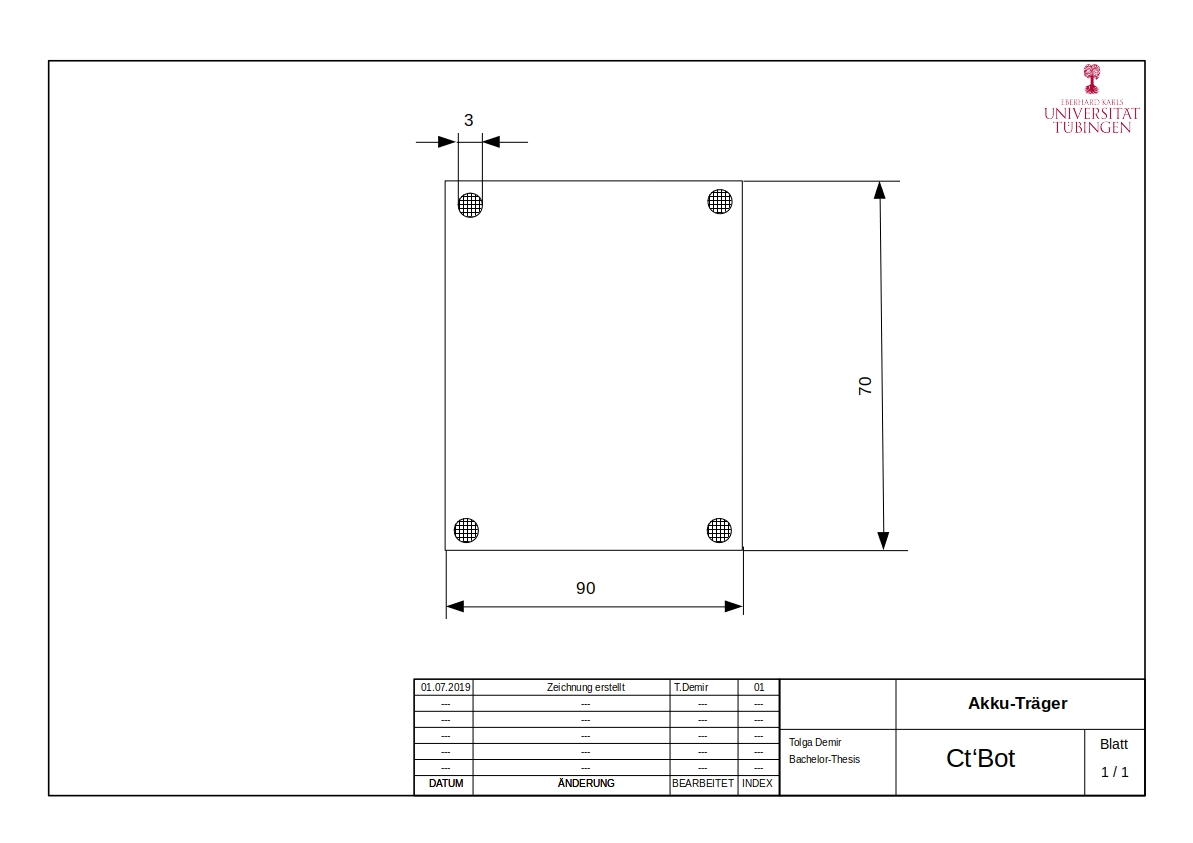
\includegraphics[angle=90,origin=c, scale= 0.7]{images/Zeichnung_Akku.jpg}
	\section{PCB-Layout}
	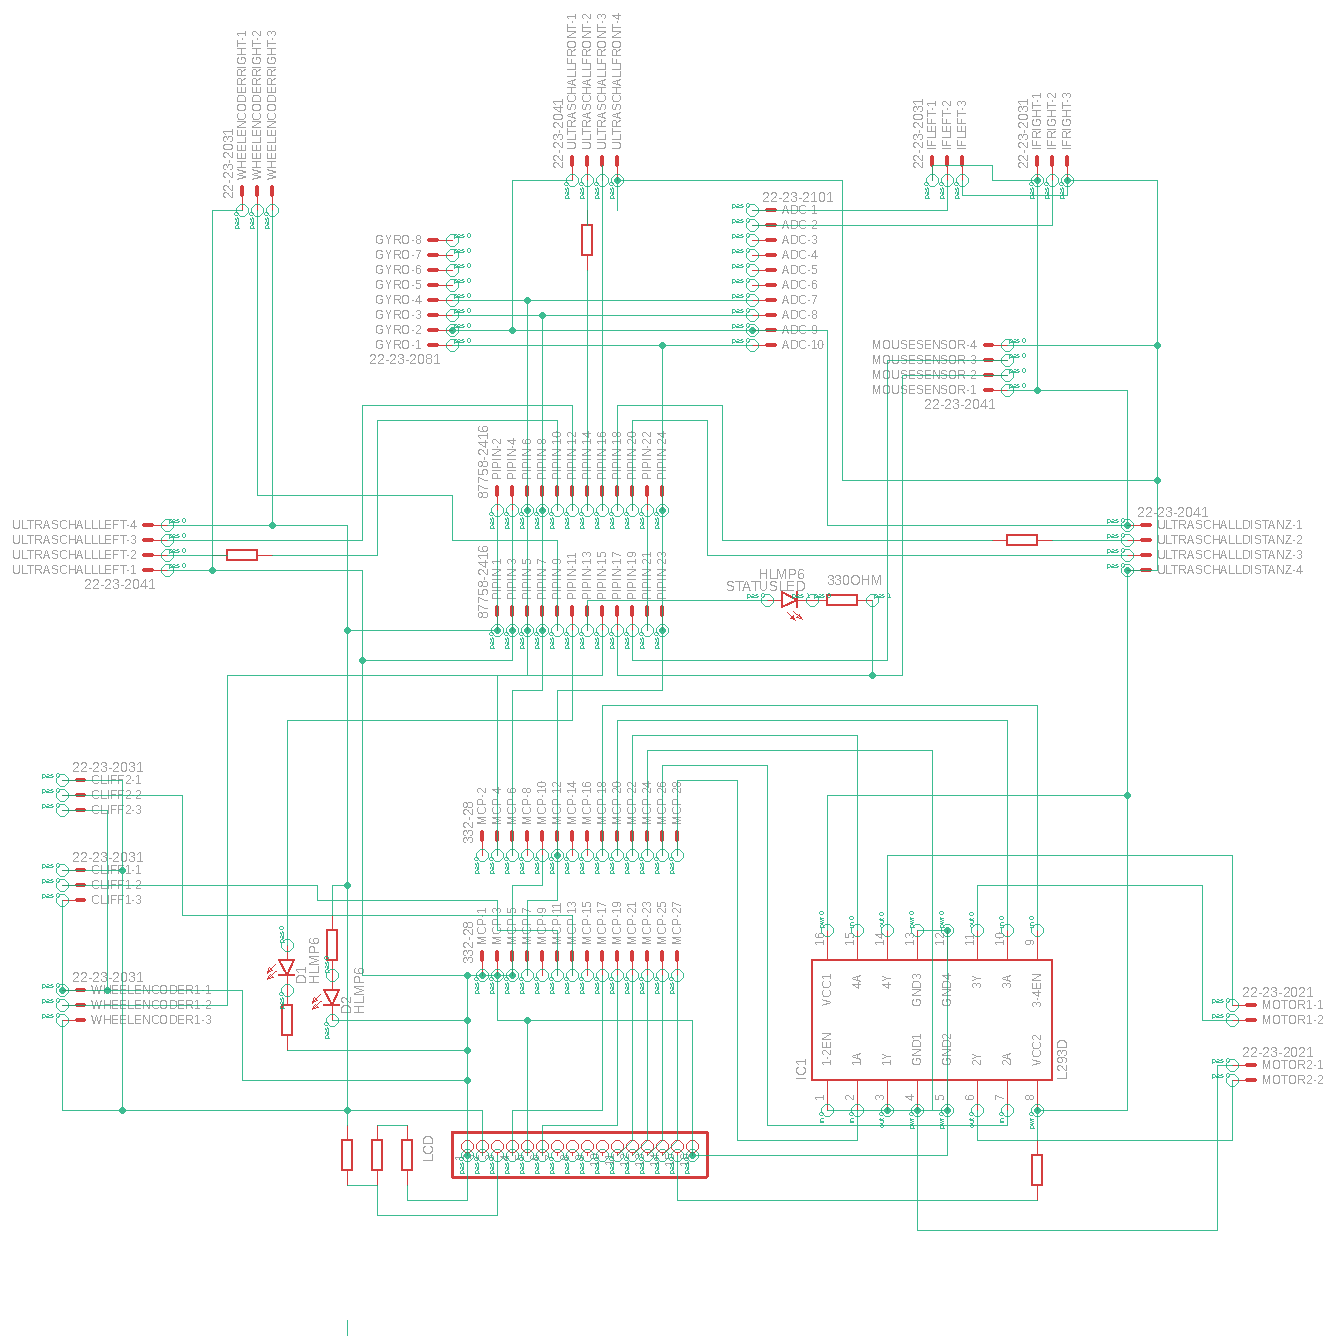
\includegraphics[angle=0,origin=c, scale= 0.75]{images/Layout.png}
	\section{PCB-Bestückung}
	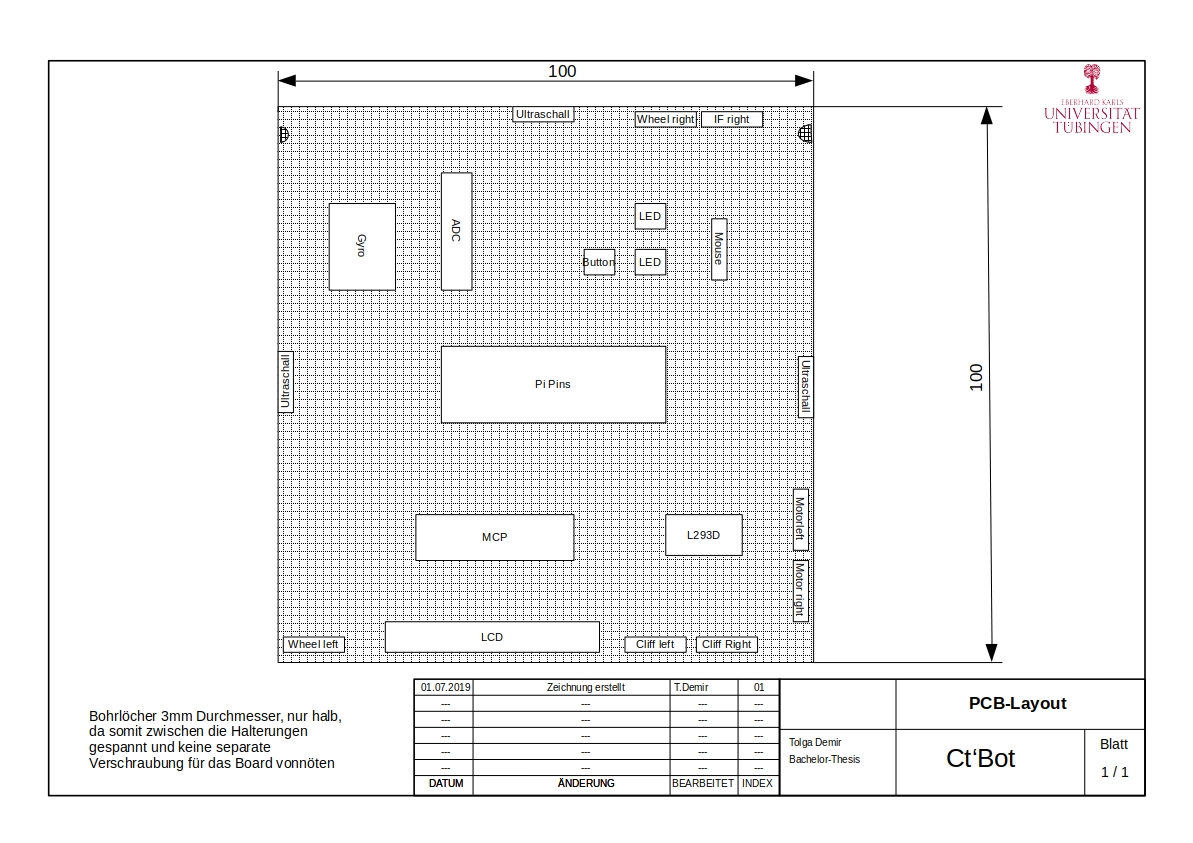
\includegraphics[angle=90,origin=c, scale= 0.7]{images/PCB-Layout.jpg}
	
	\chapter{Pin-Belegung}
	\section{Pinbelegung an der Pi}
	
	\begin{center}
		\begin{tabular}{|cc|c|c|}
			\hline
			Pin 	&BCM		& Function 		& Bauteil\\
			\hline
			2		&3			& I2C - SDA		& ADC , Gyro, MCP23017 (daran LCD, Buttons) \\
			3 		&5			& I2C - SCL		& ADC , Gyro, MCP23017 (daran LCD, Buttons)\\
			4		&7			& Freier Pin	& Ultraschall-Dist-Sens Rechts ECHO\\
			17		&11 		& Freier Pin	& Ultraschall-Dist-Sens Rechts TRIG	\\
			27		&13 		& Freier Pin	& Ultraschall-Dist-Sens Front ECHO	\\
			22		&15 		& Freier Pin	& Ultraschall-Dist-Sens Front TRIG	\\
			10		&19 		& SPI0 - MI		& 	\\
			9		&21 		& SPI0 - MO		& Button		\\
			11		&23 		& SPI0 - CL		& Wheel-Encoder Rechts		\\
			5		&29 		& Freier Pin	& Ultraschall-Dist-Sens Links ECHO		\\
			6		&31 		& Freier Pin	& Ultraschall-Dist-Sens Links TRIG	\\
			13		&33 		& Freier Pin	& Mouse-Sensor Data	\\	
			19		&35 		& Freier Pin	& Mouse-Sensor Clock	\\
			26		&37 		& Freier Pin	& Status LED\\
			14		&8 			& UART - TXD	& 	intern blockierter PIN\\
			15		&10 		& UART - RXD	&  	intern blockierter PIN\\
			18		&12 		& Freier Pin	& 	\\
			23 		&16 		& Freier Pin	& Motor-Chip Pin 15 - Driver-In0 for Mot2	\\
			24		&18 		& Freier Pin	& Motor-Chip Pin 10- Driver-In1 for Mot2	\\
			25		&22 		& Freier Pin	& Motor-Chip Pin 9 - EN for Mot2	\\
			8		&24 		& SPI0 - CE		& 	\\
			7		&26 		& SPI1 - CE		&  	\\
			12		&32 		& Freier Pin	& Wheel-Encoder Links	\\
			16		&36 		& Freier Pin	& Motor-Chip Pin 7 - Driver-In1 for Mot1	\\
			20		&38 		& SPI1 - MO		& Motor-Chip Pin 2 - Driver-In0 for Mot1		\\
			21		&40 		& SPI1	- CL	& Motor-Chip Pin 1 - EN for Mot1	\\
			\hline
		\end{tabular}
	\end{center}
	Die Pinbelegung orientiert sich an der physischen Verteilung der Pins auf der Pi (BCM-Layout). Vorsicht: Hier wird BCM genutzt, die Python Scripts verwenden jedoch BOARD-Layout. \\
	Von 24 frei programmierbaren Pins sind 17 in Benutzung, davon 2 für I2C-Kommunikation. 
	
	\section{Pinbelegung am MCP}
	Die Zählung beginnt am ersten Pin auf der oberen Seite, links. Der erste "freie" Pin ab den Funktions-Pins trägt somit die 1. danach ist die obere Seite belegt bis 8 und dann wird umgehend gezählt. Damit ist der Pin 9 der Pin auf der unteren Seite, ganz rechts und Pin 16 der Pin in der Mitte auf der unteren Seite. 
	
	\begin{center}
		\begin{tabular}{|c|c|}
			\hline
			Pin 	& Bauteil\\
			\hline
			1 - 6		&  frei\\
			7		& Cliff-Sensor links\\
			8		& Cliff-Sensor rrechts\\
			9		& LCD D7		\\
			10		& LCD D6 	\\
			11		& LCD D5		\\
			12		& LCD D4	\\
			13		& LCD E	\\	
			14		& LCD RS	\\
			15-16		& 	frei\\
			\hline
		\end{tabular}
	\end{center}
	
	\section{Pinbelegung am AD-Converter}
	Pinbelegung wie Aufdruck auf Bauteil, dh. von 0-3, starten ab Mitte.
	
	\begin{center}
		\begin{tabular}{|c|c|}
			\hline
			Pin 	& Bauteil\\
			\hline
			0-1		& 	frei\\
			2 		& IF-Sensor rechts\\
			3		& IF-Sensor links\\
			\hline
		\end{tabular}
	\end{center}
	
	\chapter{Installationsanleitung}
	Nachdem die Hardware des Roboters fertiggestellt wurde, muss die Software installiert werden. Dies geschieht durch Installation einer Rasbian Version und dem Einrichten dieser, gefolgt von der Installation versch. Python Bibliotheken und dem Framework selbst. 
	\section{Raspbian}
	Raspbian ist eine speziell für die Raspberry Pi zugeschnittene Linux Variante. Grob baut Sie auf Ubuntu auf und verzichtet auf einige der großen Programme und Treiber, insb. jener für Grafik. \\
	Raspbian lässt sich entweder direkt auf einer SD-Karte fertig installiert kaufen oder auf der offiziellen Website\\ https://www.raspberrypi.org/downloads/raspbian/ \footnote{Abgerufen am 01.07.2019 um 14:00 Uhr}
	herunterladen. Für ungeübter User empfiehlt sich hierbei die Noobs Version, welche die neueste Raspbian Version einfach zur Verfügung stellt. Für eine genaue Installationsanleitung empfiehlt sich hier das Einsteiger-Forum von Raspbian https://www.raspberrypi.org/documentation/installation/installing-images/README.md \footnote{Abgerufen am 01.07.2019 um 14:00 Uhr}
	.
	
	\subsection{Raspbian einrichten}
	Beim grundsätzlichen Einrichten des Betriebssystem sollte man der Einleitung im oben genannten Link folgen. Es sollte aber auf jeden Fall der Nutzername und das zugehörige Passwort geändert werden. Dies kann über die Konsole mit dem Befehl 'raspi-config' geschehen. \\
	
	\subsection{I2C und Kamera}
	Es muss die Kamera und der I2C-Kanal aktiviert werden. Dies geschieht im Terminal mit dem Befehl 'sudo raspi-config'. Danach öffnet sich ein Konfigurationsfenster. Hier muss unter der Punkt Interface-Optionen ausgewählt werden. In diesem Unterpunkt findet man die Menüs zu I2C und Kamera. Diese jeweils aktivieren und bestätigen. Die Pi muss danach neu gestartet werden. 
	
	\subsection{VNC-Server}
	Danach sollte ein VNC-Server installiert werden um Zugriff auf die Pi zu erhalten. Eine gute Anleitung findet sich auch wieder auf der offiziellen Website der Pi Foundation:\\
	https://www.raspberrypi.org/documentation/remote-access/vnc/ \footnote{Abgerufen am 01.07.2019 um 14:00 Uhr}
	
	
	\subsection{WLan-Access-Point}
	Ein WLan-Access-Point erleichtert den Zugriff auf die Pi. Diese stellt fortan ein WLan zur Verfügung auf das jedes externe Gerät zugreifen kann. \\
	Eine Anleitung hierzu findet sich erneut auf der offizielen Seite:\\
	https://www.raspberrypi.org/documentation/configuration/wireless/access-point.md\footnote{Abgerufen am 01.07.2019 um 14:00 Uhr}
	
	\subsection{Update and Upgrade}
	Vor und nach jeder Installation sollte im Terminal ein Update erzwungen werden. Dies passiert durch den Befehl ' sudo apt-get update' und ' sudo apt-get upgrade'. Ebenso sollte zu Beginn ein großes Update erfolgen durch den Befehl ' sudo apt-get dist-upgrade'. Nach diesen Befehlen empfiehlt sich weiterhin das Kommando ' sudo apt-get autoremove' und 'sudo apt-get autoclean' um veraltete Pakete zu entfernen. 
	
	\section{Python Bibliotheken}
	
	Für die Funktionsfähigkeit des Frameworks werden Python Bibliotheken benötigt, welche nicht in der Standartinstallation enthalten sind. Diese werden im Terminal durch den Befehl 'sudo pip install (BIBLIOTHEKNAME HERE)' installiert.\\
	Folgende Pakete werden benötigt: 
	\begin{center}
		\begin{itemize}
			\item PIL
			\item CV
			\item numpy
			\item Tkinter
			\item smbus
			\item Adafruit\_ADS1x15
		\end{itemize}
	\end{center}
	Je nach verwendeter Python Version (2 oder 3) können die Installationsnamen variieren. So heißt PIL für Python2 Pillow und CV ist zu finden unter open-cv oder opencv-python. Sollte die Installation der Pakete scheitern, so empfiehlt es sich hier nachzusehen, wie die Namen für die Installation aufgelöst werden müssen. 
	
	\section{PyBot-Framework}
	Das Herzstück der Software ist das Python-Framework. Dieses lässt sich über GitHub auf die eigene Pi clonen. Die Daten findet man unter https://github.com/Nitzsch/PyBot \footnote{Abgerufen am 02.07.2019 um 15:00 Uhr}\\
	Nachdem das Framework heruntergeladen wurde, sollte die Pin-Belegung im Unterordner Drivers an den eigenen Roboter angepasst werden. Danach lässt sich über die Ausführung des Scripts View der Roboter im Nutzer-Interface starten und steuern. \\
	Beim Ausprobieren wünscht der Autor viel Spaß und Erfolg. 
	
	\cleardoublepage
	
	
	%%%%%%%%%%%%%%%%%%%%%%%%%%%%%%%%%%%%%%%%%%%%%%%%%%%%%%%%%%%%%%%%%%%%%%%%%%%%%
	%%% Bibliographie
	%%%%%%%%%%%%%%%%%%%%%%%%%%%%%%%%%%%%%%%%%%%%%%%%%%%%%%%%%%%%%%%%%%%%%%%%%%%%%
	
	\addcontentsline{toc}{chapter}{Literaturverzeichnis}
	
	\bibliographystyle{alpha}
	\bibliography{mylit}
	%% Obige Anweisung legt fest, dass BibTeX-Datei `mylit.bib' verwendet
	%% wird. Hier koennen mehrere Dateinamen mit Kommata getrennt aufgelistet
	%% werden.
	
	
	
\end{document}
